% Typ des Dokuments
\documentclass[abstracton, a4paper, 12pt]{scrreprt}

% Encoding (utf8)
\usepackage[utf8]{inputenc}
\usepackage[T1]{fontenc}

% Silbentrennung (Neu-Deutsch)
\usepackage[ngerman]{babel}

% Literaturverzeichnis (Deutsch)
\usepackage{bibgerm}
% Spezialseiten (Literarturverzeichnis, Abbildungsverzeichnis, usw.) in Inhaltsverzeichnis anzeigen
\usepackage[nottoc]{tocbibind}

% Farben
\usepackage{color}
\usepackage[table]{xcolor}
\definecolor{darkgreen}{rgb}{0,0.6,0}
\definecolor{darkgrey}{rgb}{0.5,0.5,0.5}
\definecolor{grey}{rgb}{0.8,0.8,0.8}
\definecolor{lightgrey}{rgb}{0.95,0.95,0.95}
\definecolor{mauve}{rgb}{0.58,0,0.82}

% Schriften
\usepackage{pifont}
\newcommand{\tick}{\ding{51}\hspace{0.2cm}}
\newcommand{\cross}{\ding{55}\hspace{0.2cm}}

% Grafiken
\usepackage[pdftex]{graphicx}
\usepackage{epsfig}
% Umfliessen von Text um Tabellen und Bilder
\usepackage{wrapfig}

% Grafiken korrekt positionieren
\usepackage{float}
\restylefloat{figure}
\usepackage[section]{placeins}
\usepackage{subfigure}
% Zahlen verwenden für Subfigure counter
\renewcommand{\thesubfigure}{(\arabic{subfigure})}

% Hyperlinks und URLs
\usepackage[hyphens]{url}
\usepackage{hyperref}
\hypersetup{
   colorlinks,%
   citecolor=blue,%
   filecolor=blue,%
   linkcolor=blue,%
   urlcolor=blue
}
\urlstyle{same}

% Absatz
\setlength{\parindent}{0pt} % Absatzeinzug
\setlength{\parskip}{10pt} % Absatzabstand

% Glossar
\usepackage[toc]{glossaries}
\makeglossaries

% Kontrolle über Listen-Eigenschaften
\usepackage{enumitem}

% Abstaende bei Ueberschriften
\usepackage{titlesec}
% \titlespacing*{command}{left}{before-sep}{after-sep}[right-sep]
\titlespacing{\section}{0em}{12pt}{3pt}
\titlespacing{\subsection}{0em}{10pt}{2pt}
\titlespacing{\subsubsection}{0em}{8pt}{0em}

% TODO Kommentare
\usepackage{todonotes}

%%%%%%%%%%%%%%%%%%%%%%%%%%%%%%%%%%%%%%%%%%%%%%%%%%%
% Kopf- und Fusszeile
%%%%%%%%%%%%%%%%%%%%%%%%%%%%%%%%%%%%%%%%%%%%%%%%%%%
% Seitenränder
\usepackage[inner=2.2cm,outer=2.2cm,top=1.7cm,bottom=1.7cm,includeheadfoot]{geometry}

% Kopf- und Fusszeile mit Linien
\usepackage[automark,headsepline,footsepline]{scrpage2}

\pagestyle{scrheadings}
% Kopf- und Fusszeile auch bei Kapitel- und Partsanfangsseiten
\renewcommand*{\chapterpagestyle}{scrheadings}
\renewcommand*{\partpagestyle}{scrheadings} 

% Kopf- und Fusszeile leeren
\clearscrheadfoot

% Inhalt der Kopfzeile
\ihead{\footnotesize{\leftmark}}

% Inhalt der Fusszeile
\ifoot{\footnotesize{Gamified Mobile App für die Verbesserung von OpenStreetMap}}
\ofoot{\footnotesize{\thepage}}

% MakeUppercase überschreiben, um Grosschreibung in Kopfzeile für Spezialseiten zu deaktivieren (Achtung böser Hack!)
\renewcommand*\MakeUppercase[1]{#1}

%%%%%%%%%%%%%%%%%%%%%%%%%%%%%%%%%%%%%%%%%%%%%%%%%%%
% Tabellen
%%%%%%%%%%%%%%%%%%%%%%%%%%%%%%%%%%%%%%%%%%%%%%%%%%%
% Für Tabellen, welche über mehrere Seiten gehen
\usepackage{longtable}

% Padding links und rechts von Zelle
\setlength{\tabcolsep}{5px}
% Padding oben und unten (mittels arraystretch)
\renewcommand{\arraystretch}{1.3}

% Variabeln für Tabellenbreiten definieren
% 2-spaltige Tabelle
\newlength{\twocelltabwidth}
\setlength{\twocelltabwidth}{\textwidth}
\addtolength{\twocelltabwidth}{-4\tabcolsep - 3px} % subtrahiere 4x Padding (\tabcolsep) und 3 Rahmen

% 3-spaltige Tabelle
\newlength{\threecelltabwidth}
\setlength{\threecelltabwidth}{\textwidth}
\addtolength{\threecelltabwidth}{-6\tabcolsep - 4px} % subtrahiere Padding (\tabcolsep) und Rahmen

% 4-spaltige Tabelle
\newlength{\fourcelltabwidth}
\setlength{\fourcelltabwidth}{\textwidth}
\addtolength{\fourcelltabwidth}{-8\tabcolsep - 5px} % subtrahiere Padding (\tabcolsep) und Rahmen

%%%%%%%%%%%%%%%%%%%%%%%%%%%%%%%%%%%%%%%%%%%%%%%%%%%
% Syntaxhighlighter
%%%%%%%%%%%%%%%%%%%%%%%%%%%%%%%%%%%%%%%%%%%%%%%%%%%
% Syntaxhighlighter (benoetigt color und xcolor package)
\usepackage{listings}
\renewcommand{\lstlistingname}{Code-Ausschnitt}
 
\lstset{ %
  language=HTML,                % the language of the code
  basicstyle=\footnotesize,           % the size of the fonts that are used for the code
  numbers=left,                   % where to put the line-numbers
  numberstyle=\tiny\color{darkgrey},  % the style that is used for the line-numbers
  stepnumber=1,                   % the step between two line-numbers. If it's 1, each line will be numbered
  numbersep=5pt,                  % how far the line-numbers are from the code
  backgroundcolor=\color{white},  % choose the background color. You must add \usepackage{color}
  showspaces=false,               % show spaces adding particular underscores
  showstringspaces=false,         % underline spaces within strings
  showtabs=false,                 % show tabs within strings adding particular underscores
  frame=single,                   % adds a frame around the code
  rulecolor=\color{darkgrey},        % if not set, the frame-color may be changed on line-breaks within not-black text (e.g. commens (green here))
  tabsize=2,                      % sets default tabsize to 2 spaces
  captionpos=b,                   % sets the caption-position to bottom
  breaklines=true,                % sets automatic line breaking
  breakatwhitespace=false,        % sets if automatic breaks should only happen at whitespace
  title=\lstname,                   % show the filename of files included with \lstinputlisting;
                                  % also try caption instead of title
  keywordstyle=\color{blue},          % keyword style
  commentstyle=\color{darkgreen},       % comment style
  stringstyle=\color{mauve},         % string literal style
  escapeinside={\%*}{*)},            % if you want to add a comment within your code
  morekeywords={*,...}               % if you want to add more keywords to the set
}

% Javascript Syntaxhighliting
\lstdefinelanguage{JavaScript} {
	morekeywords={
		break,const,continue,delete,do,while,export,for,in,function,
		if,else,import,in,instanceOf,label,let,new,return,switch,this,
		throw,try,catch,typeof,var,void,with,yield
	},
	sensitive=false,
	morecomment=[l]{//},
	morecomment=[s]{/*}{*/},
	morestring=[b]",
	morestring=[d]'
}
\lstset{
	frame=tb,
	framesep=5pt,
	basicstyle=\footnotesize\ttfamily,
	showstringspaces=false,
	keywordstyle=\ttfamily\bfseries\color{blue},
	identifierstyle=\ttfamily,
	stringstyle=\ttfamily\color{mauve},
	commentstyle=\color{darkgreen},
	rulecolor=\color{darkgrey},
	xleftmargin=5pt,
	xrightmargin=5pt,
	aboveskip=\bigskipamount,
	belowskip=\bigskipamount
}

% Inline Code-Formatierung
\newcommand{\inlinecode}{\texttt}

% Silbentrennung
\hyphenation{Web-app-li-ka-tion}
\begin{document}

% -----------------------------------------
% HEAD
% -----------------------------------------
% Titelseite
\title{Gamified Mobile App für die Verbesserung von OpenStreetMap}
\author{Jürg Hunziker\\jhunzike@hsr.ch
		\and
		Stefan Oderbolz\\soderbol@hsr.ch}
\date{22. Dezember 2012}

\begin{titlepage}

% Logos
\begin{figure}[H]
\subfigure{
\includegraphics[width=200px]{images/titlepage/logo-hsr}}
\hfill
\raisebox{37px}{\subfigure{
\includegraphics[width=125px]{images/titlepage/logo-bitforge}}}
\end{figure}

\vspace{2.2cm}

\begin{center}
{ \Large
	% Titel
	\textbf{Gamified Mobile App für die Verbesserung von OpenStreetMap}
	\vspace{1cm}

	% Arbeitstyp / Schule
	\textbf{Bachelorarbeit}
	\vspace{1cm}

	Abteilung Informatik \\[0.2cm]
	HSR Hochschule für Technik Rapperswil
	\vspace{1cm}

	% Semester
	Herbstsemester 2012/13
}
\end{center}
\vspace{2.3cm}


\begin{table}[H] 
\centering 
\begin{tabular}{p{0.19\twocelltabwidth}p{0.4\twocelltabwidth}}
Autoren: & \textbf{Jürg Hunziker} \newline
\textbf{Stefan Oderbolz} \\ 
Betreuer: & \textbf{Prof. Stefan Keller} \\ 
Projektpartner: & \textbf{Reto Senn}, bitforge AG Zürich \\ 
Experte: & \textbf{Claude Eisenhut} \\ 
Datum: & \textbf{21. Dezember 2012} \\ 
\end{tabular}
\end{table}

\end{titlepage}

% Seitennummerierung mit roemischen Zeichen
\pagenumbering{roman}

% Glossar (muss vor Body inkludiert werden, damit Referenzen funktionieren)
% Glossar
\newglossaryentry{API} {
	name = API,
	description = {Application Programming Interface, Schnittstelle für die Programmierung}
}

\newglossaryentry{OAuth} {
	name = OAuth,
	description = {OAuth ist ein offenes Protokoll, das eine standardisierte, sichere API-Autorisierung erlaubt\cite{oauth}}
}

\newglossaryentry{CRUD} {
	name = CRUD,
	description = {Das Akronym CRUD beschreibt die 4 Standardoperationen einer Datenbank: \textbf{C}reate, \textbf{R}ead, \textbf{U}pdate, \textbf{D}elete\cite{crud}}
}

\newglossaryentry{AntTarget} {
	name = Ant Target,
	description = {Das Buildautomatisierungs-Tool Ant nennt die einzelnen Schritte eines Builds \emph{Target}. Targets sind eine Sammlung von semantisch zusammengehörigen Tasks. Sie können Abhängigkeiten zu anderen Targets aufweisen, welche dann als Vorbedingung zuerst ausgeführt werden\cite{ant-target}}
}

\newglossaryentry{Cloud} {
	name = Cloud,
	description = {Als Cloud oder Cloud-Computing (\emph{Wolke}) bezeichnet man die Gesamtheit aller Dienste, welche ortsunabhängig im Internet angeboten werden. Dies können zum Beispiel Datenspeicher, Server oder Datenbanken oder schlicht Rechenleistung sein. Der grosse Vorteil der Cloud ist, dass sie sehr leicht skalierbar ist, so dass man  die Leistungen dynamisch an den Bedarf angepassen kann\cite{cloud}}
}

\newglossaryentry{HeadlessBrowser} {
	name = headless Browser,
	description = {Bei einem \emph{headless Browser} handelt es sich um einen Browser, welcher ohne grafische Benutzeroberfläche auskommt. Häufig werden sie dazu verwendet, um Serverjobs, welche auf den Browser angewiesen sind, auszuführen}
}

\newglossaryentry{WebApp} {
	name = Web-App,
	description = {Der Begriff Web-App (von der englischen Kurzform für web application), bezeichnet im allgemeinen Sprachgebrauch Apps für mobile Endgeräte wie Smartphones und Tablet-Computer, die über einen in das Betriebssystem integrierten Browser aus dem Internet geladen und so ohne Installation auf dem mobilen Endgerät genutzt werden können\cite{webapp}}
}

\newglossaryentry{REST} {
	name = REST,
	description = {Representational State Transfer\cite{rest} ist ein Programmierparadigma, welches besagt, dass sich der Zustand einer Webapplikation als Ressource in Form einer URL beschreiben lässt. Auf eine solche Ressourcen können folgende Befehle angewendet werden: \inlinecode{GET}, \inlinecode{POST}, \inlinecode{PUT},\inlinecode{PATCH}, \inlinecode{DELETE}, \inlinecode{HEAD} und \inlinecode{OPTIONS}.
	HTTP ist ein Protokoll welches REST implementiert}
}

\newglossaryentry{Git} {
	name = Git,
	description = {Git ist ein verteiltes Versionsverwaltungssystem für Dateien. Ursprünglich wurde es für die Entwicklung des Linux Kernels entwickelt}
}

\newglossaryentry{ci} {
	name = Continuous Integration,
	description = {Unter dem Begriff \emph{Continuous Integration}\cite{cont-integration} beschreibt die Idee, dass Änderungen an einer Software schnell eingebracht werden sollen. Dazu zählt, dass diese in einem Versionsverwaltungs-Tool eingetragen und durch automatisierte Tests geprüft werden}
}

\newglossaryentry{Bootstrapping} {
	name = Bootstrapping,
	description = {Bootstrapping wird der Prozess genannt, der auf einem einfachen System ein komplexeres System aktiviert\cite{bootstrapping}. Dadruch wird das System ermächtigt, sich selbst zu starten. Deshalb wird Bootstrapping auch Lösung für das Henne-Ei-Problem genannt}
}

\newglossaryentry{POI} {
	name = POI,
	description = {Abkürzung für Point of Interest. Dies ist ein allgemeiner Begriff für einen Ort mit irgendeiner Bedeutung, sei es eine Schule, Kirche, Bushaltestelle oder sonst etwas von besonderem Interesse}
}

\newglossaryentry{Mapper} {
	name = Mapper,
	description = {Personen welche auf OpenStreetMap die Karten ergänzen und pflegen, nennen sich selbst \emph{Mapper}}
}

\newglossaryentry{App-Store} {
	name = App-Store,
	description = {Ein App-Store ist eine Verkaufsplattform eines Betriebssystemherstellers für Smartphones. Beispielsweise Google Play für Android, Apple App Store für iOS}
}

\newglossaryentry{Camera API} {
	name = Camera API,
	description = {Das Camera API ist eine Spezifikation vom W3C\cite{camera-api}, welches den Zugriff auf die Kamera und die Bilder eines Endgerätes beschreibt}
}

\newglossaryentry{Microloader} {
	name = Microloader,
	description = {Der Microloader ist dafür zuständig, beim Starten einer Sencha Touch Applikation alle verwendeten Ressourcen (wie JavaScript- oder CSS-Files) zu laden}
}

\newglossaryentry{Local Storage} {
	name = Local Storage,
	description = {Beim Local Storage handelt es sich um einen Key-Value Speicher des Browser in welchen Daten einer Webseite persistiert werden können}
}

\newglossaryentry{Node} {
	name = Node,
	description = {Ein Node ist das grundlegenste Objekt in OpenStreetMap, es wird durch seine Attribute (genannt \glspl{Tag}) genauer bestimmt. Nodes können Teil eines \gls{Way} sein}
}

\newglossaryentry{Way} {
	name = Way,
	description = {Ein Weg oder eine Strasse wird in OpenStreetMap als \emph{Way} bezeichnet. Es handelt sich dabei um eine Serie von miteinander verbundenen Nodes}
}

\newglossaryentry{Relation} {
	name = Relation,
	description = {Eine Relation stellt eine Verbindung zwischen anderen OSM-Objekten dar. Relationen werden meist gebraucht über übergeordnete Beziehungen darzustellen, welche sich nicht direkt geografisch ergibt. Beispielsweise können alle Bushaltestellen einer Buslinie über eine Relation miteinander verknüpft sein}
}

\newglossaryentry{Tag} {
	name = Tag,
	description = {Ein Tag bezeichnet ein Attribut eines \glslink{Node}{Nodes}. Es besteht aus einem Namen und einem Wert. Ein \gls{Node} kann beliebig viele Tags beinhalten}
}

\newglossaryentry{OpenStreetMap} {
	name = OpenStreetMap,
	description = {OpenStreetMap ist ein freies Projekt, das für jeden frei nutzbare Geodaten sammelt (Open Data). Mit Hilfe dieser Daten können Weltkarten errechnet oder Spezialkarten abgeleitet werden sowie Navigation betrieben werden}
}

\newglossaryentry{Gamification} {
	name = Gamification,
	description = {Unter Gamification versteht man das Hinzufügen von Spiel-Elementen in einem nicht spieltypischen Kontext}
}

% TODO Liste
% Titel auch in Kopfzeile anzeigen
\markboth{Todo list}{Todo list}
\listoftodos

% Impressum & Aenderungsverlauf
\chapter*{Impressum und Revision}
% Titel auch in Kopfzeile anzeigen
\markboth{Impressum und Revision}{Impressum und Revision}

% Impressum
\section*{Impressum}
\begin{table}[H] 
\centering 
\begin{tabular}{|p{0.35\twocelltabwidth}|p{0.65\twocelltabwidth}|}
\hline 
\textbf{Autoren:} & Jürg Hunziker (\url{jhunzike@hsr.ch}) \newline
Stefan Oderbolz (\url{soderbol@hsr.ch}) \\ 
\hline 
\textbf{Dokument erstellt:} & 05.10.2012 \\ 
\hline 
\textbf{Letzte Aktualisierung:} & 21.12.2012 \\ 
\hline 
\end{tabular}
\end{table}

Dieses Dokument wurde mit \LaTeX{} erstellt.

% Aenderungsverlauf
\section*{Änderungsverlauf}

\begin{longtable}{|p{0.15\threecelltabwidth}|p{0.65\threecelltabwidth}|p{0.2\threecelltabwidth}|}
\hline 
\textbf{Datum} & \textbf{Änderungen} & \textbf{Bearbeiter} \\ 
\hline 
05.10.2012 & Dokumententwurf erstellt & Stefan Oderbolz \\ 
\hline 
10.10.2012 & Leaflet Komponente dokumentiert & Jürg Hunziker \\ 
\hline 
01.12.2012 & Abstract erstellt & Jürg Hunziker \\ 
\hline 
02.12.2012 & Backend-Administration & Jürg Hunziker \\ 
\hline
05.12.2012 & Server-Setup hinzugefügt & Stefan Oderbolz \\ 
\hline 
06.12.2012 & Entwurf des Management Summary & Stefan Oderbolz \\ 
\hline 
\end{longtable} 

% Erklaerung
\chapter*{Erklärung}
% Titel auch in Kopfzeile anzeigen
\markboth{Erklärung}{Erklärung}

Ich erkläre hiermit,
\begin{itemize}
\item dass ich die vorliegende Arbeit selber und ohne fremde Hilfe durchgeführt habe, ausser derjenigen, welche explizit in der Aufgabenstellung erwähnt ist oder mit dem Betreuer schriftlich vereinbart wurde,
\item dass ich sämtliche verwendeten Quellen erwähnt und gemäss gängigen wissenschaftlichen Zitierregeln korrekt angegeben habe.
\end{itemize}

\vspace{3cm}

\begin{tabular}{p{0.5\twocelltabwidth}p{0.5\twocelltabwidth}}
Ort, Datum: & Ort, Datum: \\ 
\end{tabular} 

\vspace{1cm}

\begin{tabular}{p{0.5\twocelltabwidth}p{0.5\twocelltabwidth}}
Name, Unterschrift: & Name, Unterschrift: \\ 
\end{tabular} 

% Abstract
% Neue Seite beginnen
\cleardoublepage

% Stil des Abstract-Titels veraendern
\renewcommand{\abstractname}{{\Huge\bfseries Abstract}}
% Titel auch in Kopfzeile anzeigen
\markboth{Abstract}{Abstract}

\begin{abstract}
% Kopf- und Fusszeile auch auf Abstractseite
\thispagestyle{scrheadings}

Das Ziel dieser Arbeit war das Erstellen einer cross-platform \gls{WebApp} zur Behebung von Fehlern in den OpenStreetMap-Daten.

Mit der App lassen sich verschiedene Typen von Fehlern beheben.
Dies kann zum Beispiel ein fehlendes Geschwindigkeitslimit bei einer Strasse oder ein Point of Interest ohne Namen sein.

Die gemachten Lösungsvorschläge der Benutzer werden dann von anderen Benutzern validiert.
Damit lässt sich die Qualität der Daten sicherstellen.
Wurde ein Lösungsvorschläg genügend oft positiven bewertet, so gilt dieser als akzeptiert. 
Solche Korrekturen werden dann zurück zu OpenStreetMap geschickt und somit die Karte für alle verbessert.

Um einen Anreiz zu bieten, die App längerfristig zu verwenden, wurden verschiedene Game-Elemente eingebaut.
So lassen sich beispielsweise mit dem Lösen von Fehlern Punkte sammeln und Auszeichnungen gewinnen.
Zusätzlich kann man sich über eine Highscore mit den anderen Spielern vergleichen.

Dieses Konzept, welches auch als Gamification bezeichnet wird, wurde im Bericht noch weiter beschrieben.
Es wurden weitere mögliche Elemente, welche in diesem Zusammenhang sinnvoll wären, untersucht und dokumentiert.

\end{abstract}


% Management Summary
\chapter*{Management Summary}
\thispagestyle{scrheadings}
% Titel auch in Kopfzeile anzeigen
\markboth{Management Summary}{Management Summary}

\todo[inline]{Management Summary schreiben}

\section*{Ausgangslage}
Das OpenStreetMap-Projekt beinhaltet eine sehr grosse Menge an Daten, welche frei zugänglich ist.
Für die Pflege dieser Daten ist es daher naheliegend auf unterstützende Software zurückzugreifen.
Zu diesem Zweck gibt es eine Reihe von Applikationen, welche sich grob in zwei Kategorien einteilen lassen:
Editoren und Qualitätssicherung

Mit den Editoren lässt sich direkt oder indirekt die OpenStreetMap-Karte verändern und ergänzen.
Die Qualitätssicherung hat sich zum Ziel gesetzt fehlende oder falsche Daten aufzuspüren.
Diese werden dann entweder automatisiert korrigiert oder übersichtlich dargestellt, um eine manuelle Korrektur zu ermöglichen.

Einige Tools wie Keepright\footnote{\url{http://keepright.ipax.at/}} oder Osmose\footnote{\url{http://osmose.openstreetmap.fr/map/}} berechnen aus den Karten-Rohdaten die vorhanden Fehler.
Dazu werden einige Heuristiken verwenden oder einfache Plausibilitätsprüfungen durchgeführt.
Typische Fehler aus diesen Quellen sind \gls{POI}s ohne Namen oder Wege ohne eingetragenen Typ.

\begin{figure}[H]
	\centering
	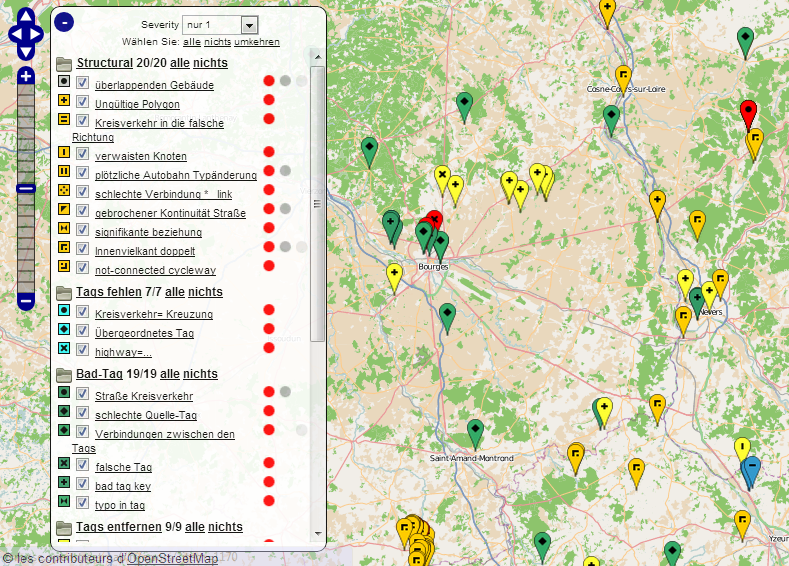
\includegraphics[scale=0.4]{images/managementsummary/osmose-screenshot}
	\caption{Anzeige von generierten Fehlern in Osmose}
	\label{image-osmose-screenshot}
\end{figure}

Andere Lösungen setzen darauf, dass Fehler manuell von einer Person erfasst werden. Dadurch ist es möglich den Fehler detaillierter zu beschreiben. 
So gibt es Navigationsgeräte-Herstellen welche die Daten aus OpenStreetMap zur Routenberechnung verwenden und dabei ihren Benutzern ermöglichen falsche Routen zu melden.
Falls ein \gls{Mapper} einen Fehler markieren will, so kann er dies direkt in den Metadaten der Karte hinterlegen. Jedes Objekt auf der Karte (Punkte, Wege und Relationen) kann durch beliebige, sogenannte  \emph{Tags} ergänzt werden.
Um auf einem Objekt Fehler zu markieren, hat sich die Community darauf geeinigt \inlinecode{FIXME}-Tags zu verwenden.

Quellen für solche Fehler sind beispielsweise OpenStreetBugs\footnote{\url{http://openstreetbugs.schokokeks.org/}} oder die \inlinecode{FIXME}-Tags aus Keepright.

\section*{Ergebnisse}
Das Ziel, eine cross-platform fähige \gls{WebApp} zu erstellen mit geeignetem Backend für die Verwaltung der Daten wurde klar erreicht.
Die App bietet alle Grundfunktionalität welche nötig ist um Fehler anzuzeigen, zu lösen und gegebene Lösungen zu validieren.
Daneben sind einige Elemente der Gamification implementiert. So kann man beispielsweise durch das Lösen von Fehlern Punkte (sogenannte \emph{koins}) sammeln und sich über eine Highscore, mit anderen Spielern messen.
Zudem gibt es für speziellen Einsatz Auszeichnungen zu gewinnen.

\begin{figure}[H]
	\centering
	
\includegraphics[scale=0.6]{images/gamification/gamification-badges}
	\caption{Auszeichnungen in Kort}
	\label{image-kort-badges}
\end{figure}

Der Bereich der Gamification ist aber sehr offen und lässt Raum für viele weitere Konzepte. Schlussendlich ist klar, dass \textsc{Kort} noch ein grosses Stück davon entfernt ist ein "`echtes"' Game zu sein.

Das Themengebiet der Gamification bietet viele Ansätze um eine normalerweise \emph{uninteressante} Aufgabe spannend zu machen.
Dadurch erhalten diese Aufgaben einen ganz neuen Reiz und sprechen direkt den Spieltrieb des Menschen an.
Konkret auf OpenStreetMap angewendet, finden sich auch dort beliebtere und weniger beliebte Aufgaben.
Da es sich bei dabei zusätzlich um eine Community von (grösstenteils) freiwilligen Personen handelt, verschärft sich dieses Problem.
Das Problem der mangelnden Ressourcen kann dabei am effektivsten bekämpft werden, indem zusätzliche Personen für das Thema begeistert werden.
Es ist wichtig, die Einstiegsschwelle tief zu halten und auch einem unerfahrenen Benutzer Werkzeuge zu geben, die einen gewissen Spass vermitteln.

\subsection*{Frontend}
Das Frontend basiert auf dem HTML5/JavaScript Framework Sencha Touch 2 und orientiert sich vom Look and Feel an einer iPhone-App.
Die App bietet für die verschiedenen Funktionen unterschiedliche Tabs an, auf welchen der Benutzer Fehler beheben oder prüfen und die Highscore oder sein Profil anschauen kann.

\begin{figure}[H]
\subfigure{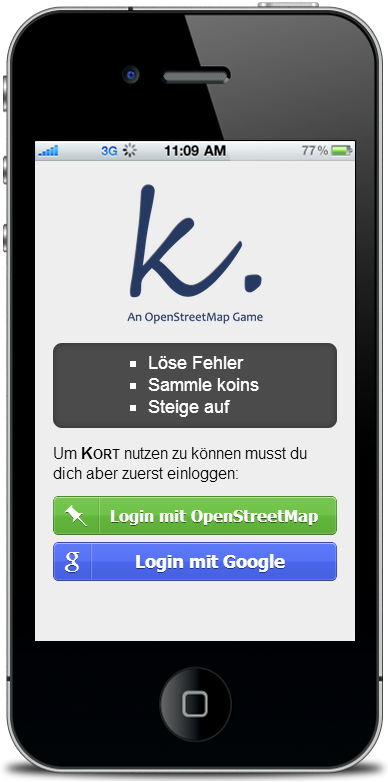
\includegraphics[width=0.3\textwidth]{images/screenshots/kort-screenshot-login}}
\hfill
\subfigure{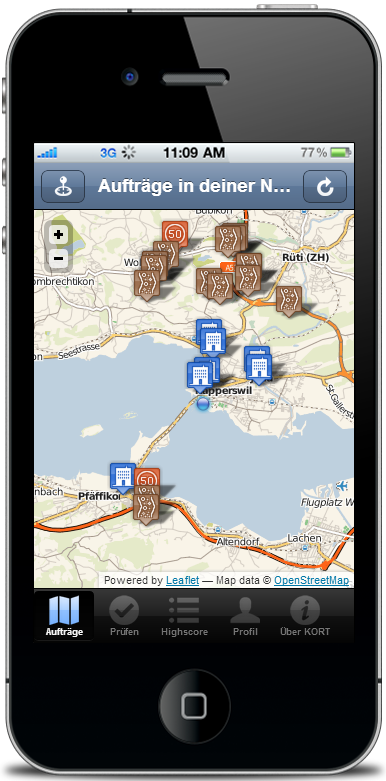
\includegraphics[width=0.3\textwidth]{images/screenshots/kort-screenshot-bugmap}}
\hfill
\subfigure{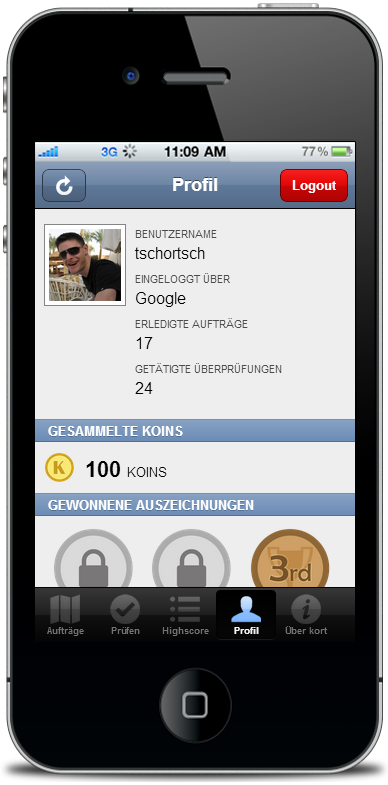
\includegraphics[width=0.3\textwidth]{images/screenshots/kort-screenshot-profile}}
\caption{Kort App}
\label{image-kort-screenshots}
\end{figure}

Für die Authentifizierung kommt \gls{OAuth} zum Einsatz.
Dir Standard sorgt dafür, dass sich der Benutzer mit einem bereits bestehenden Benutzerkonto bei \textsc{Kort} anmwelden kann.
Derzeit wird dafür der OAuth-Provider \emph{Google} verwendet.

\subsection*{Backend}
Das Backend ist in PHP geschrieben und basiert auf der Kommunikation über \gls{REST}-Schnittstellen.
Die eigenen Schnittstellen sind alle mit dem Slim-Framework\footnote{\url{http://www.slimframework.com/}} erstellt.
Da die Datenbank und der Webserver auf zwei verschiedenen Servern laufen, bietet auch die Datenbank eine REST-Schnittstelle an, über welche sich beliebige SQL-Abfrage absetzen lassen.
Diese flexible Aufteilung ermöglicht es sehr einfach die Systeme umzuziehen oder weitere hinzuzufügen.

\section*{Ausblick}
Die App hat ein grosses Potential um Personen, welche sich bislang nicht mit der Thematik OpenStreetMap befasst haben, für das Projekt zu begeistern. 
Dabei ist es wichtig, dass dieses Zielpublikum nicht aus den Augen verloren wird, weshalb in diesem Bereich noch viele Verbesserung möglich sind.

Ganz allgemein ist es wichtig die Robustheit und Geschwindikeit der App zu verbessern. 
Gerade weil es sich um eine \gls{WebApp} handelt, ist dies besonders kritisch. 
Im Idealfall sollte sich die App nicht von einer nativen App unterscheiden.
Es ist zu prüfen, ob es sich lohnt, die App native zu builden\footnote{z.B. mit Apache Cordova oder Sencha Packager}.
Dies hätte den weiteren Vorteil, dass die App über die bekannten \gls{App-Store}s zum User gebracht werden kann.

Beim Login wäre es wünschenswert noch weitere \gls{OAuth}-Dienste anzubieten, um so weitere Personen anzusprechen und die Akzeptanz zu steigern.
Schliesslich verfügt nicht jeder über ein Google-Konto oder ist bereit sich über dieses anzumelden.
Mögliche Dienste wären dabei Facebook, Twitter oder OpenStreetMap selbst, welche alle \gls{OAuth}-Dienste anbieten.

In der Konzeption der App haben wir uns ursprünglich das Ziel gesetzt, das \gls{Camera API} zu verwenden. 
So könnten Benutzer beim Eintragen von Lösungsvorschlägen direkt ein \emph{Fotobeweis} anbringen. 
Dies würde die Validierung der eingetragenen Lösungen für andere Benutzer vereinfachen.

Als zusätzliche Motivation könnten zeitlich begrenzte Aktionen durchgeführt werden.
Dies soll Benutzer animieren die App immer wieder zu verwenden. 
Mögliche Aktionen wären beispielsweise die Konzentration auf einen Fehlertyp (\emph{"Gib allen Restaurants in deiner Umgebung einen Namen und erhalte diese Woche die spezielle Restaurant-Auszeichnung"}) oder auf eine Region (\emph{"Korrigiere jeden Tag im Dezember Fehler in Zürich und erhalte die Zürich-Silvester-Auszeichnung"}).
Bestehende Spieler können beispielsweise über Push-Notifikationen über solche Aktionen oder sonstige Neuerungen informiert werden.
Dies soll Benutzer regelmässig animieren, die App zu verwenden.

Um längerfristig die App am laufen zu halten ist es unumgänglich weitere Fehlertypen und -quellen einzubinden. 
Keepright bietet zwar eine grosse Menge an Fehlerdaten, jedoch ist nur ein geringer Teil davon für unsere App nutzbar.

Die Bekanntheit der App muss durch geeignete Massnahmen gesteigert werden, dazu gehört die Integration von Social Media Diensten wie Facebook und Twitter.
Dies kann einerseits genutzt werden um Werbung zu machen, anderseits können Benutzer auch auf ihre gewonnenen Auszeichnungen aufmerksam machen und so andere bereits bestehende Benutzer dazu animieren diese Auszeichnungen ebenfalls zu gewinnen.

% Inhaltsverzeichnis
\tableofcontents

% -----------------------------------------
% BODY
% -----------------------------------------
% Neue Seite beginnen (um Seitennummerierung zurückzusetzen)
\cleardoublepage

% Seitennummerierung mit arabischen Zeichen
\pagenumbering{arabic}

% Einleitung
% Titel auch in Kopfzeile anzeigen
\markboth{Teil I. Einleitung}{Teil I. Einleitung}
\part{Einleitung}
% Informationen zum Projekt
\chapter{Informationen zum Projekt}
\label{informationen-projekt}


\section{Problemstellung}
\gls{OpenStreetMap} ist ein freies Projekt, welches jedermann ermöglicht, Kartendaten anzuzeigen und zu editieren.
Durch diesen öffentlichen Charakter ist es nicht ausgeschlossen, dass fehlerhafte bzw. unvollständige Daten eingetragen werden.

Aus diesem Grund entstand die Idee mit einer mobilen Applikation eine Möglichkeit anzubieten, Fehler anzuzeigen und zu korrigieren.
Um die Motivation für die Verwendung der App längerfristig zu erhalten, soll diese mit Spiel-Elementen versehen werden.

\section{Aufgabenstellung}
Im Rahmen dieser Arbeit soll eine HTML5 \gls{WebApp} entwickelt werden, welche es ermöglicht, unvollständige bzw. fehlerhafte Daten in der \gls{OpenStreetMap}-Datenbank zu korrigieren oder zu vervollständigen.

Die App soll nicht als herkömmlicher Editor implementiert werden, sondern einen gewissen Gamecharakter aufweisen.
Dieser zeichnet sich dadurch aus, dass die Benutzer für ihre Änderungsvorschläge belohnt werden.
So können sie beispielsweise in der Rangliste (Highscore) aufsteigen oder Abzeichen (Badge) gewinnen.
Dieses Prinzip ist unter dem Stichwort \emph{Gamification} bekannt.
Das ist die Anwendung von Game-Elementen in einer nicht-typischen Spieldomäne.
Es soll untersucht werden, ob und wie sich dies für \gls{OpenStreetMap} umsetzen lässt.

Eingetragene Änderungsvorschläge können anschliessend von weiteren Benutzern kontrolliert und bewertet werden.
Mehrfach validierte Änderungen sollen ins \gls{OpenStreetMap}-Projekt zurückgeführt werden.

Mit der Integration von Social Media-Diensten (Facebook, Twitter) soll die Bekanntheit der App gefördert und die Motivation der Benutzer gesteigert werden.

\section{Ziele}
In der Aufgabenstellung der Arbeit wurden folgende Ziele definiert:
\begin{itemize}
	\item Erstellen einer Cross-platform HTML5 WebApp mit JavaScript
	\item Einsatz von JavaScript APIs zur Verwendung von Hardwarekomponenten (z.B. Kamera, GPS)
	\item Es soll geprüft werden, ob die WebApp auch als native App für die Plattformen iOS und Android zur Verfügung gestellt werden kann 
	\item Als Basis sollen Daten und Webdienste des \gls{OpenStreetMap}-Projekts verwendet werden
	\begin{itemize}
		\item Quellen für bekannte Fehler: OSM Bug Reports, FIXME und TODO
		\item Unterstützung von POI-, Linestring- und Polygon-Objekten
	\end{itemize}
	\item Verwendung einer vorhanden User-Basis für die Authentifizierung (OAuth)
	\item Integration von Social Media zum Austausch von Aktivitäten
	\item Konzept für Gamification von \gls{OpenStreetMap} erarbeiten
	\begin{itemize}
		\item Highscores / Rankings
		\item Badges / Achievements
		\item Aufgaben mit verschiedenen Schwierigkeitsstufen
	\end{itemize}
	\item Verschiedene Modi
	\begin{itemize}
		\item Erfassen von Daten, Aufnahme von Fotos (ortsbezogen)
		\item Verifikation von eingegebenen Daten (ortsunabhängig)
	\end{itemize}
	\item Das User Interface soll primär auf Deutsch erstellt werden. Es sollen jedoch Vorkehrungen getroffen werden, um eine Übersetzung einfach zu ermöglichen (Internationalisierung).
\end{itemize}

\section{Rahmenbedingungen}
\begin{itemize}
\item Es gelten die Rahmenbedingungen, Vorgaben und Termine der HSR
\item Die Projektabwicklung orientiert sich an einer iterativen, agilen Vorgehensweise. Als Vorgabe dient dabei Scrum, wobei bedingt durch das kleine Projektteam gewisse Vereinfachungen vorgenommen werden. Meilensteine werden bezüglich Termin und Inhalt mit dem Betreuer vereinbart.
\item Die Kommunikation in der Projektgruppe, in der Dokumentation und an den Präsentationen erfolgt auf Deutsch.
\item Je nach Zeitplanung soll ein Video gemäss den Vorgaben des Studiengangs realisiert und publiziert werden.
\end{itemize}

\section{Vorgehen / Aufbau der Arbeit}
\todo[inline]{Vorgehen beschreiben}
Vorgehen: Was wurde gemacht? In welchen Teilschritten? Risiken der Arbeit? Wer war involviert (Durchführung, Entscheide usw.)? Details in anderen Kapiteln.
Einführung in die Problem- und Aufgabenstellung. Übersicht über die übrigen Teile der Abgabe. 


Die Arbeit ist in vier Teile gegliedert. Im ersten Teil erfolgt eine Einleitung mit allgemeinen Informationen zum Projekt und dessen Umsetzung (siehe Kapitel \ref{informationen-projekt} und \ref{umsetzung}). Darauf folgt eine theoretische Einführung in das Thema (siehe Kapitel \ref{einfuehrung}) sowie unserer verwendeten Infrastruktur (siehe Kapitel \ref{infrastruktur}). Der dritte Teil behandelt die erstellten Arbeitsresultate (siehe Kapitel XXXXXXXXXX) und im vierten Teil befinden sich Informationen zum Projektmanagement (siehe Kapitel \ref{projektmanagement} und \ref{projektmonitoring}).

Neben diesem Dokument umfasst diese Arbeit eine implementierte Webapplikationen, welche im Internet verfügbar ist. Der dazugehörige Source Code ist ebenfalls frei im Internet zugänglich sowie auf der beigelegten CD zu finden.

\begin{table}[H]
\centering
\begin{tabular}{|p{0.3\twocelltabwidth}|p{0.7\twocelltabwidth}|}
\hline 
\textbf{Arbeitsresultat} & \textbf{URL} \\ 
\hline 
\textsc{Kort} (WebApp) & \url{http://kort.herokuapp.com} \\ 
\hline 
Repository & \url{https://github.com/odi86/kort} \\ 
\hline 
\end{tabular}
\label{arbeitsresultate}
\caption{Übersicht der Arbeitsresultate}
\end{table} 


% Umsetzung
\chapter{Umsetzung}
\label{umsetzung}

\section{Stand der Technik}
Da es sich bei \brand{OpenStreetMap} um ein globales Projekt handelt, gibt es zahlreiche Anstrengungen die Karte besser zu machen.
Neben konventionellen Editoren gibt es auch Tools, welche sich explizit der Findung und Behebung von Fehlern spezialisiert haben.
Ein Beispiel davon ist der \brand{NoName-Layer} von Simon Poole\footnote{\url{http://wiki.openstreetmap.org/wiki/NoName}}. Dieser färbt Strassen, welche fälschlicherweise keinen Namen haben, rot ein.
Daneben gibt es Dienste, welche Fehlerdaten sammeln und diese zur Verbesserung anbieten, wie beispielsweise \brand{KeepRight}\footnote{\url{http://www.keepright.at/}} oder \brand{OpenStreetBugs}\footnote{\url{http://openstreetbugs.schokokeks.org/}}.

Die Gemeinsamkeit dieser Werkzeuge findet sich darin, dass sie bereits ein gewisses Interesse an \brand{OpenStreetMap} und am Editieren der Karte voraussetzen.
Karten-Fehler sind jedoch typische Beispiele welche sich durch die Mithilfe von möglichst vielen Personen lösen lassen (sogenanntes \emph{Crowdsourcing})\todo{Crowdsourcing ins Glossar}.
Die Voraussetzung für ein erfolgreiches Crowdsourcing ist es, möglichst kleine Hürden zu haben und einfach zu lösende Aufgaben bereit zu stellen.

Das Konzept der \gls{Gamification} bietet sich daher an.
Dabei werden Spiel-Elemente in eine Applikation eingebaut und dadurch die Motivation der Benutzer gesteigert, diese Applikation längerfristig zu verwenden.
Es gibt bereits einige Projekte, welche sich mit der \gls{Gamification} von \brand{OpenStreetMap} beschäftigen\footnote{\url{http://wiki.openstreetmap.org/wiki/Games\#Gamification_of_map_contributions}}.

\brand{MapRoulette}\footnote{\url{http://wiki.openstreetmap.org/wiki/MapRoulette}} stellt dem Benutzer eine \emph{Challange}, welche es zu lösen gibt.
Ein Beispiel einer solchen Challange ist \emph{Connectivity}\footnote{\url{https://oegeo.wordpress.com/2012/10/29/new-maproulette-challenge-connectivity-bugs/}}, bei welcher Strassen, die sehr nahe beieinander liegen verbunden werden sollen.
Der Benutzer hat die Wahl, ob er den Fehler korrigiert, ignoriert oder als \emph{false positive} markiert.
Wenn der Benutzer einen Fehler gelöst hat, wird ihm zufällig ein weiterer Fehler angezeigt.
Die Challange ist dann fertig, wenn alle Fehler einer Kategorie behoben sind.
Durch die Weiterleitung auf den nächsten Fehler entsteht ein beinahe endloses Spiel. Jede erledigte Aufgabe hat dabei den Charakter eines Levels.

Im Rahmen der \emph{Operation Cowboy}\footnote{\url{http://wiki.openstreetmap.org/wiki/DE:Operation_Cowboy}} wurden unter anderem auch mit \brand{MapRoulette} über 2000 Routing-Fehler pro Tag behoben\footnote{\url{https://twitter.com/opcowboy/status/272438199769501696}}.

\section{Vision}
Die \gls{WebApp} \kort{} bietet dem Benutzer eine einfache Oberfläche, Fehler zu lokalisieren.
Das Zielpublikum hat keinerlei Vorwissen über Karten oder \brand{OpenStreetMap}.
Da die App als Spiel konzipiert ist, werden dem Benutzer kleine, einfach zu lösende Aufgaben gestellt.
Diese Aufgaben beziehen sich alle auf Fehler in den Karten-Daten.

Für das Lösen solcher Aufgaben, gewinnt er Punkte und kann so in der Highscore aufsteigen.
Für besondere Leistungen werden dem Benutzer dabei auch Auszeichnungen verliehen.
Dieser Mix sorgt dafür, dass der Benutzer die App immer wieder öffnet, um weitere Korrekturen vorzunehmen.

Als Alternative zum Beantworten von Fragen, hat ein Benutzer die Möglichkeit, die Antworten von anderen Spielern zu validieren.
Dazu soll er die gegebenen Antworten als richtig oder falsch markieren.
Erreicht eine Antwort genügend Stimmen, welche deren Richtigkeit bestätigen, gilt diese als abgeschlossen und kann anschliessend als Korrektur an \brand{OpenStreetMap} gesendet werden.

Durch die Implementation als cross-platform \gls{WebApp}, kann diese auf allen gängigen mobilen Betriebssystemen verwendet werden.

\section{Resultate der Arbeit}
Wir konnten fast alle gesetzten Ziele erreichen.
\kort{} erfüllt alle Anforderungen an eine moderne \gls{WebApp}.
Nach dem Login über \gls{OAuth} werden dem Benutzer Fehler in seiner Umgebung auf der Karte angezeigt.

Um das Spiel zu starten kann der Benutzer eine beliebige Aktionen durchführen.
Wenn er beispielsweise einen Fehler auswählt, indem er auf dessen Markierung tippt, wird er gefragt, ob er die Lösung für den Fehler kennt.
Dadurch soll die Neugier des Spielers geweckt werden.
Alle abgeschlossenen Aufgaben werden mit Punkten (sogenannten \emph{Koins}) belohnt.\todo{komischer Satz}

Die Spielmechanik ist denkbar einfach, so dass das Spiel auch nur sekunden- aber auch  minutenlang gespielt werden kann.
Der Benutzer erhält sofort ein Feedback und kann verfolgen, wie er sich gegenüber seinen Mitspielern verbessert.
Eine zusätzliche Motivation wird über Auszeichnungen geschaffen.
Diese werden für spezielle Leistungen vergeben und erscheinen auf der eigenen Profil-Seite.\todo{komischer Satz}

Wir konnten einige Gamificationkonzepte direkt in der App umsetzen.
Um das Spiel für möglichst viele Benutzer attraktiv zu machen, muss aber ein noch detaillierteres Konzept ausgearbeitet werden.
Gerade mit den Badges lassen sich verschiedene Spielertypen ansprechen.
Auch Schwierigkeitsstufen oder zusätzliche Berechtigungen für erfahrene Benutzer können den längerfristigen Erfolg der Applikation erhöhen.

Auf der technischen Seite haben wir erfolgreich ein System entwickelt, welches stets mit neuen Fehlern "`gefüttert"' wird.
Die Architektur ist so flexibel gewählt, dass sich beinahe beliebig Komponenten hinzufügen oder entfernen lassen.
Dies stellt sicher, dass zukünftig noch weitere Fehlerdatenquellen in \kort{} integriert werden können.

\section{Schlussfolgerungen und Ausblick}
Leider konnten nicht alle Punkte aus der Aufgabenstellung erfüllt werden.
Wir hatten das Ziel, dass Benutzer neben einer textuellen Antwort auch ein Bild hochladen können, um einen Beweis für eine Fehlerkorrektur zu liefern.
Dabei sind wir jedoch an einer technischen Limite des verwendeten Frontend-Frameworks \brand{Sencha Touch 2} gescheitert.
Des weiteren sollten soziale Medien wie Facebook und Twitter integriert werden, um eine breitere Öffentlichkeit zu erreichen.
Im Verlaufe der Arbeit haben sich die Prioritäten diesbezüglich aber geändert.

Als letzter offener Punkt bleibt noch das Zurückschreiben der Korrekturen zu \brand{OpenStreetMap}.
Da wir damit beschäftigt waren unser eigenes System fertig zu stellen, konnten wir dies schlussendlich aus Zeitgründen nicht mehr implementieren.

Die App in der jetzigen Form ist also in sich geschlossen. Die getätigten Korrekturen werden in der eigenen Datenbank abgelegt, jedoch noch nicht zu \brand{OpenStreetMap} zurückgesendet.

Wir mussten in dieser Arbeit feststellen, dass zuerst eine solide Basis erstellt werden muss, auf der dann Weiterentwicklungen stattfinden können.
Ursprünglich haben wir uns erhofft, tiefer in die Thematik der \gls{Gamification} einzusteigen und die App als "`echtes"' Game zu gestalten.

Wenn unsere App trotzdem mithelfen kann, einzelne Benutzer für das \glslink{Mapper}{Mappen} zu begeistern, dann haben wir unser  Ziel mehr als erreicht.

% Neue Seite beginnen
\cleardoublepage

% Projektdokumentation
% Titel auch in Kopfzeile anzeigen
\markboth{Teil II. Projektdokumentation}{Teil II. Projektdokumentation}
\part{Projektdokumentation}
% Infrastruktur
\chapter{Infrastruktur}
\label{infrastruktur}

\section{Architektur}

Das Gesamtsystem setzt sich aus insgesamt vier Komponenten zusammen: die Datenbank, der Webserver, die Fehlerquelle und das Zielsystem von OpenStreetMap. 
Die einzelnen Komponenten sind über \gls{REST}-Schnittstellen miteinander verbunden. 
Dabei sind das Zielsystem (OpenStreetMap) und die Fehlerquelle (Keepright, siehe Kapitel \ref{datenquellen}) Fremdsysteme, bei welchen die Schnittstellen gegeben waren. 
Unsere eigenen Server haben wir entsprechend angepasst und auch via REST zugänglich gemacht.

\begin{figure}[H]
	\centering
	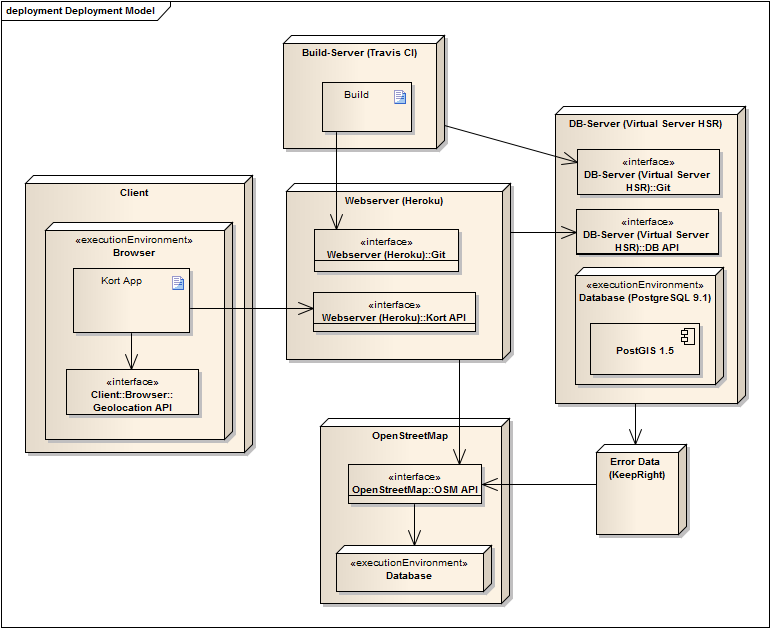
\includegraphics[width=\textwidth]{images/uml/deployment_diagram}
	\caption{Gesamtübersicht der Systeme}
	\label{deplyoyment-diagram}
\end{figure}


\section{Datenbankserver}

Beim Datenbankserver handelt es sich um einen virtuellen Server, den uns die Hochschule für Technik Rapperswil (HSR) zur Verfügung gestellt hat für die Dauer dieser Arbeit.

\begin{table}[H]
\centering
\begin{tabular}{|p{0.25\twocelltabwidth}|p{0.75\twocelltabwidth}|}
\hline 
\small{\textbf{Art des Servers}} & Virtueller Server \\
\hline 
\small{\textbf{Betriebsystem}} & Ubuntu 12.04 (LTS) \\
\hline 
\small{\textbf{Zugriff}} & Root-Zugriff via SSH \\
\hline 
\small{\textbf{Installierte Software}} & PostgreSQL 9.1, PostGIS 2.0, Redmine 2.1 \\
\hline 
\end{tabular} 
\caption{Datenbankserver der Hochschule für Technik Rapperswil}
\label{infrastruktur-datenbankserver-tabelle}
\end{table}

\subsection{Backup}
\todo[inline]{Backup-Section schreiben (DB-Server)}

\section{Webserver (Heroku)}

Bei Heroku\footnote{\url{http://www.heroku.com/}} handelt es sich um einen kostenlosen Dienst, welcher für verschiedenste Plattformen eine Deploymentumgebung anbietet. 
Der Dienst hat eine Schnittstelle über welche sich automatisiert Applikationen erstellen lassen, die Datenübertragung läuft dann über \gls{git}.

\begin{table}[H]
\centering
\begin{tabular}{|p{0.25\twocelltabwidth}|p{0.75\twocelltabwidth}|}
\hline 
\small{\textbf{Art des Servers}} & Server in der \gls{Cloud} \\
\hline 
\small{\textbf{Betriebsystem}} & Ubuntu \\
\hline 
\small{\textbf{Zugriff}} & Daten via \gls{git}, Befehle via Kommandozeilen-API (Heroku Toolbelt) \\
\hline 
\small{\textbf{Installierte Software}} & Apache, kort Applikation \\
\hline 
\end{tabular} 
\caption{Server bei Heroku}
\label{infrastruktur-heroku-tabelle}
\end{table}

Die Entscheidung den Webserver von Heroku zu wählen ist dadurch begründet, dass uns dies die grösstmögliche Freiheit bietet. 
Heroku bietet bereits eine hervoragende \gls{API} welche sich über das Kommandozeilen-Toolset \emph{Heroku-Toolbelt} steuern lässt.
Dies erlaubt es beliebig viele Applikationen automatisiert zu erstellen.
Auch für den Betrieb bietet das API viele Möglichkeiten zur Fernwartung an (SSH-Zugang, Logs, Prozessorauslastung).
Alle diese Faktoren zusammen ergeben die ideale Lösung für 

\section{Deployment}
Am Deployment der Applikation sind mehrere Systeme beteiligt. 
Alle Änderungen werden von den Entwicklern via \gls{git} zu GitHub\footnote{\url{http://github.com}} übertragen. 
Auf GitHub gibt es sogenannte Hooks die man aktivieren kann. 
Dabei handelt es sich um weitere Aktionen welche durch verschiedene Ereignisse ausgelöst werden können. 
In unserem Fall haben wir einen \emph{post-commit Hook} aktiviert, welcher dem \gls{ci} Dienst Travis-CI\footnote{\url{http://travis-ci.org}} Bescheid gibt, wenn ein neue Änderungen auf GitHub eingetroffen sind.

Auf Travis läuft dann der Build, welcher durch die Konfigurationsdatei \inlinecode{.travis.yml} gesteuert ist. Darin lassen wir die Schritte sowie die Umgebung für Builds definieren. Für jede Umgebung wird dann ein separater Build ausgelöst. Somit lassen sich bequem verschiedene Versionen mit unterschiedlichen Umgebungen testen.
Daraus entsteht dann eine sogenannte Build-Matrix welche bei jedem Build durchlaufen wird (siehe Tabelle \ref{infrastruktur-build-matrix}).

Ein Travis-Build läuft immer in einer neuen virtuellen Umgebung, so dass strikt nach dem Prinzip des \emph{\gls{Bootstrapping}s} vorgegangen werden muss. Das heisst, es muss möglich sein die Applikation ohne Vorkenntnisse zu installieren, alle benötigte Software und Konfiguration muss bei jedem Build vorgenommen werden.
Dies hilft, den Installationprozess genau festzuhalten

Am Ende des Build-Vorgangs wird die \gls{WebApp} schliesslich zu Heroku übertragen. 

\begin{table}[H]
\centering
\begin{tabular}{|p{0.2\threecelltabwidth}|p{0.4\threecelltabwidth}|p{0.4\threecelltabwidth}|}
\hline 
 & \textbf{Test} & \textbf{Produktion} \\
\hline 
\textbf{PHP 5.3} & Build und Test & Build und Test \\
\hline 
\textbf{PHP 5.4} & Build, Test und Deployment auf \url{http://kort-dev.herokuapp.com} & Build, Test und Deployment auf \url{http://kort.herokuapp.com} \\
\hline 
\end{tabular} 
\caption{Build-Matrix von Travis CI}
\label{infrastruktur-build-matrix}
\end{table}

\todo[inline]{gruntjs, ant, secure ENV, }
\todo[inline]{PHPDoc, PHPCS}
\todo[inline]{Update-Service}


% Leaflet Sencha Touch Komponente
\chapter{OpenStreetMap-Daten in Sencha Touch}
\label{leaflet-sencha-komponente}

\section{Sencha Touch Map-Komponente}

Das Sencha Touch 2-Framework bietet zur Darstellung einer Karte lediglich eine Google Maps-Komponente an.
Diese ist stark auf das Google Maps API ausgerichtet und kann deshalb nicht für andere Kartendaten verwendet werden.

Um trotzdem Daten von \brand{OpenStreetMap} verwenden zu können, mussten wir eine neue Sencha Touch Map-Komponente erstellen, welche eine für diesen Zweck vorgesehene Library verwendet.

\section{Leaflet Map-Komponente}

Zur Darstellung der OSM-Daten verwendeten wir zuerst die \brand{OpenLayers}\footnote{\url{http://openlayers.org/}}-Library.
Leider mussten wir nach einiger Zeit feststellen, dass diese für unsere Zwecke zu komplex und überladen ist.

Wir haben deshalb eine Komponente erstellt, welche die \brand{Leaflet}\footnote{\url{http://leafletjs.com/}}-Library zur Darstellung der Karte verwendet.
Leaflet ist eine moderne, leichtgewichtige Karten-Library.
Sie wurde speziell für den Einsatz auf mobilen Geräten konzipiert.
Zusätzlich ist sie sehr gut dokumentiert und lässt sich einfach bedienen.

\begin{figure}[H]
	\centering
	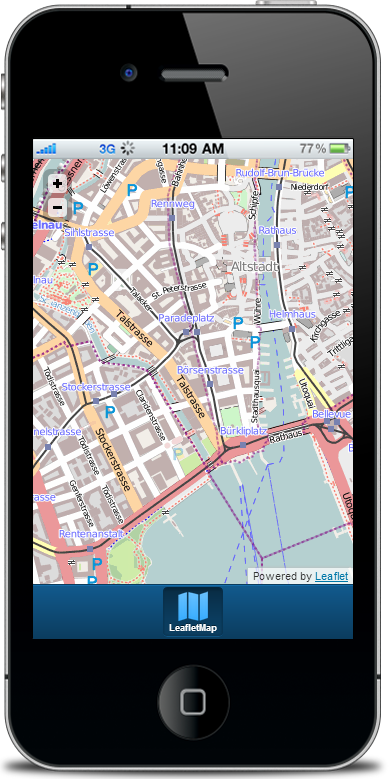
\includegraphics[scale=0.5]{images/implementation/frontend/leafletmap-screenshot}
	\caption{Ext.ux.LeafletMap-Komponente in Sencha Touch}
	\label{image-leafletmap-screenshot}
\end{figure}

\subsection{Verfügbarkeit}
Unsere Sencha Touch Komponente war zuletzt so ausgereift, dass wir uns entschieden haben, diese für die Allgemeinheit zugänglich zu machen.
Wir veröffentlichten sie deshalb unter dem Namen \brand{Ext.ux.LeafletMap} im offiziellen Sencha Market\footnote{\url{http://market.sencha.com/}}.
Sie ist verfügbar unter: \url{https://market.sencha.com/users/162/extensions/177}.

\begin{table}[H]
\centering
\begin{tabular}{|p{0.2\twocelltabwidth}|p{0.8\twocelltabwidth}|}
\hline 
\textbf{Ort} & \textbf{URL} \\ 
\hline 
Sencha Market & \url{https://market.sencha.com/users/162/extensions/177} \\ 
\hline 
GitHub & \url{https://github.com/tschortsch/Ext.ux.LeafletMap} \\ 
\hline 
\end{tabular} 
\caption{Ext.ux.LeafletMap Verfügbarkeit}
\label{leafletmap-availiblity}
\end{table}

\begin{figure}[H]
	\centering
	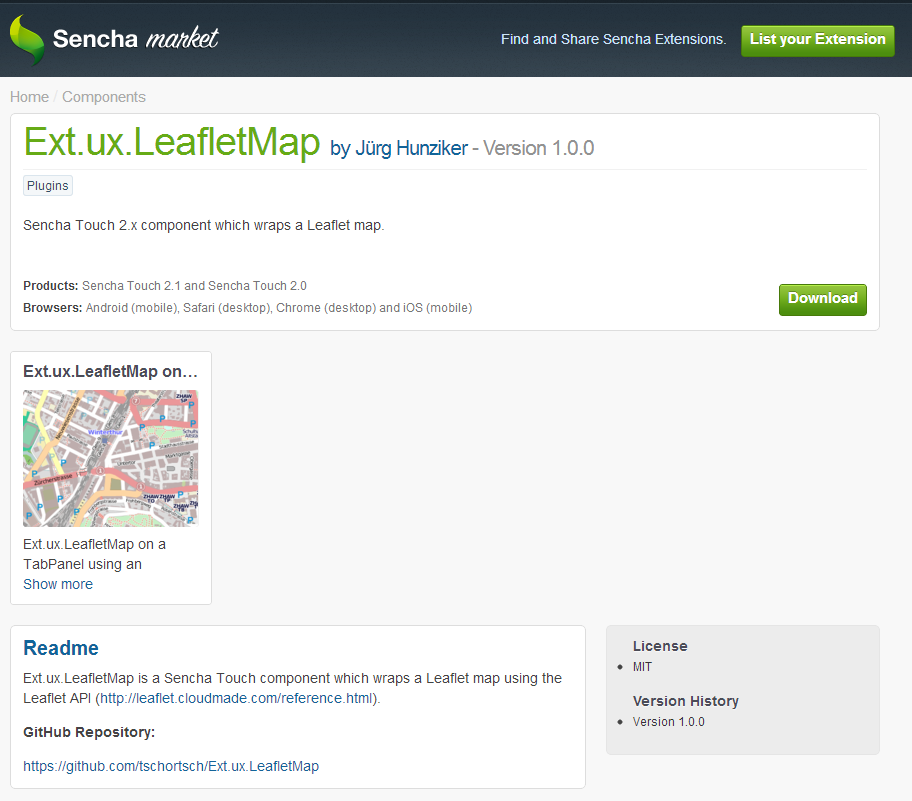
\includegraphics[scale=0.6]{images/implementation/frontend/leafletmap-sencha-market}
	\caption{Leaflet Map-Komponente im Sencha Market}
	\label{image-leafletmap-sencha-market}
\end{figure}

\subsection{Dokumentation}
Die Komponente ist durchgängig mit der Sencha-eigenen JavaScript-Dokumentationssprache \brand{JSDuck}\footnote{\url{https://github.com/senchalabs/jsduck}} dokumentiert. Die Dokumentation befindet sich unter: \url{http://kort.herokuapp.com/docs/Ext.ux.LeafletMap}.

% Gamification
\chapter{Gamification}
\label{gamification}

Unter Gamification versteht man die Verwendung von spieltypischen Elementen in einem spielfremden Kontext.
Die bekanntesten Elemente sind dabei die Punktevergabe für das Lösen von Aufgaben, die Verleihung von Badges für besonders engagierte Einsätze oder das Bereitstellen einer Highscore zum Vergleich mit anderen Benutzern.

Während unserer Arbeit hatten wir verschiedene Partner, welche uns bei der Gamification unserer Applikation unterstützen.
So ist einer unserer Industriepartner Mitinhaber der Firma bitforge AG\footnote{\url{http://bitforge.ch/}}, welche sich auf Games im mobilen Umfeld spezialisiert hat.
Er konnte uns vor und während der Entwicklung viele wertvolle Tipps zur Verbesserung des Spielgefühls geben.

\section{Gamification in Kort}
\subsection{Sprache}
Gamification findet sich nicht nur in schönen Grafiken und Spiel-Elementen.
Sie beginnt bereits bei der Sprachwahl von Texten.
Beim Lesen der Texte sollte beispielsweise eine gewisse Spannung aufgebaut werden.
Dadurch erhöht sich die Motivation die anstehende Aktion durchzuführen.

In \kort{} findet sich dafür ein Beispiel in der Button-Bezeichnung bei der Eingabe des eigenen Benutzernamens.
Zu Beginn war dieser mit "`App starten"' beschriftet.
Wir haben ihn aber später mit dem Text "`Mission beginnen!"' ersetzt.
Weiter wurde der Button grün eingefärbt, um ihn zusätzlich vom Text und vom Hintergrund abzuheben.

\begin{figure}[H]
	\centering
	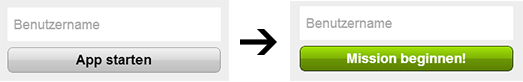
\includegraphics{images/gamification/gamification-lang-firststeps}
	\caption{Gamification - Sprache}
	\label{gamification-lang-firststeps}
\end{figure}

Neben der gewählten Ausdrucksweise sollte die Sprache dem Zielpublikum angepasst werden.
Wir mussten dafür viele Begriffe aus dem \glslink{Mapper}{Mapping}-Vokabular für unserer breite Zielgruppe mit allgemeineren Wörtern ersetzen.

\subsection{Punktesystem "`Koins"'}
Eines der wichtigsten Elemente im Spiel bildet das Punktesystem. Dieses findet sich in beinahe allen Aktionen der App wieder.
So gewinnt ein Spieler für gelöste Aufgaben oder getätigte Prüfungen eine gewisse Anzahl an sogenannten \emph{Koins}.
Über die Anzahl \emph{Koins} kann er sich wiederum in der Highscore mit den anderen Spieler messen.

\begin{figure}[H]
	\centering
	
\includegraphics[scale=0.4]{images/gamification/gamification-koin}
	\caption{Gamification - Koins}
	\label{gamification-koins}
\end{figure}

\subsection{Auszeichnungen}
Zusätzlich zu den \emph{Koins} kann ein Spieler Auszeichnungen gewinnen. Diese erhält man durch besondere Leistungen. In \kort{} sind momentan folgende Auszeichnungen implementiert:

\begin{table}[H]
\centering
\begin{tabular}{|p{0.25\twocelltabwidth}|p{0.75\twocelltabwidth}|}
\hline 
\textbf{Auszeichnungstyp} & \textbf{Beschreibung} \\ 
\hline 
Anfänger & Eine Auszeichnungen für das Lösen vom 1. Auftrag und eine für das Überprüfen der 1. Antwort. \\ 
\hline 
Platzierung & Drei Auszeichnungen für das Erreichen des 1., 2. und 3. Rangs in der Highscore. \\ 
\hline 
Aufträge & Drei Auszeichnungen für das Lösen von 10, 50 und 100 Auträgen. \\ 
\hline 
Prüfungen & Drei Auszeichnungen für 10, 10 und 1000 geprüfte Antworten. \\ 
\hline 
\end{tabular} 
\caption{Auszeichnungen in Kort}
\label{kort-badges}
\end{table}

\begin{figure}[H]
	\centering
	
\includegraphics[scale=0.7]{images/gamification/gamification-badges}
	\caption{Gamification - Badges}
	\label{gamification-badges}
\end{figure}

Das Hinzufügen von zusätzlichen Auszeichnungen ist in Abschnitt \ref{kort-additional-badges} beschrieben.

\subsection{Highscore}
Über die Highscore haben die Benutzer der App die Möglichkeit sich mit den anderen Spielern zu vergleichen.
Dazu werden sie nach Anzahl gewonnener \emph{Koins} in einer Rangliste eingestuft.

\section{Weitere mögliche Elemente}
Neben den verwendeten Gamification-Elementen in \kort{} gibt es noch eine Vielzahl weiterer Elemente, welche sich für diesen Anwendungszweck eigenen würden.
Diese konnten während der Arbeit aber nicht implementiert werden.

Daneben gibt es aber auch noch Elemente welche zwar für OpenStreetMap als Projekt interessant wären, sich jedoch nicht mit \kort{} umsetzen lassen.

\subsection{Erste Schritte}
Um den Einstieg in die Verwendung der App weiter zu vereinfachen wäre es sinnvoll beim ersten Start eine kurze Einführung anzuzeigen.
So könnte man dem Benutzer für die einzelnen Masken jeweils Tipps einblenden oder gar eine geführte Tour durch die App und deren Möglichkeiten anbieten.

Wenn der Benutzer nicht weiss, welche Möglichkeiten er hat, kann dies dazu führen, dass er schnell wieder aufgibt oder nicht das volle Potential der App ausschöpfen kann.

\subsection{Zeitlich begrenze Aktionen}
Durch das Einführen von zeitlich begrenzten Aktionen kann man Benutzer dazu motivieren die App auch nach längerer Zeit noch zu verwenden.
So könnte man Tage definieren, an denen man die doppelte Anzahl an Punkten gewinnt.
Zusätzlich könnte man Aktionen starten, bei denen man spezielle Auszeichnungen gewinnen kann.\footnote{Beispiel einer zeitlich begrenzen Aktion in \brand{OpenStreetMap}: Das \brand{big baseball project 2011} \url{http://wiki.openstreetmap.org/wiki/Big_baseball_project_2011}}

Um den Benutzer dazu zu animieren die App erneut zu starten, könnte man per Push-Meldungen auf aktuelle Aktionen, Updates oder Ereignisse aufmerksam machen.

\subsection{Weitere Auszeichnungen hinzufügen}
Bei der Auswahl an verfügbaren Auszeichnungen sollte man darauf achten, dass es für jeden Spielertyp geeignete Auszeichnungen zu gewinnen gibt.
Die verschiedenen Typen haben eine ganz andere Herangehensweise und müssen deshalb auch mit verschiedenen Belohnungen motiviert werden.
Eine Einteilung von verschiedenen Spielertypen wird auf \brand{Gamasutra}\footnote{\url{http://www.gamasutra.com/view/feature/6474/personality_and_play_styles_a_.php}} beschrieben.

Es gibt bereits eine Liste von möglichen Badges im Wiki von OpenStreetMap\footnote{\url{https://wiki.openstreetmap.org/wiki/Badges}}.

\subsection{Verschiedene Highscores}
Durch das Bereitstellen von verschiedenen Highscores (Bsp. Regional, Nach Fehlertyp), gibt man allen Benutzern die Chance, irgendwo den ersten Platz zu erreichen.
Dadurch verhindert man eine mögliche Demotivation beim Vergleich mit Langzeitspielern, welche bereits eine grosse Anzahl an Punkten gesammelt haben.

\subsection{Erfahrene Spieler}
Man könnte als Belohnung für viele gelöste Fehler die Berechtigungen des Benutzers erhöhen.
So könnte beispielsweise seine Stimme bei einer Überprüfung einer Lösung doppelt zählen.
Dieses Prinzip wird auch von der Frage/Antwort-Plattform \brand{Stack Overflow}\footnote{\url{http://stackoverflow.com/}} angewendet.

\begin{figure}[H]
	\centering
	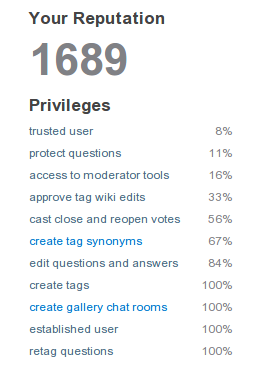
\includegraphics[scale=0.7]{images/gamification/so-privileges}
	\caption{Zusätzliche Berechtigungen bei StackOverflow}
	\label{gamification-so-privileges}
\end{figure}

Um erfahrene Spieler nicht zu unterfordern, könnte man ihm beim Erreichen einer gewissen Punktzahl, Fehler anzeigen, welche schwieriger zu lösen sind.
Wichtig ist es dabei, dass das Spiel nicht plötzlich vorbei ist.
Auch der Spieler der bereits die meisten Punkte hat, muss noch eine Motivation haben die App weiter zu verwenden.

\subsection{Einbinden in Apple Game Center}
Apple bietet mit dem \brand{Game Center} einen zentralen Ort an, Punkte und Auszeichnungen von Game-Apps zu speichern.
Dadurch entsteht für die Spieler die Möglichkeit sich direkt mit anderen Spielern und Kollegen, die ebenfalls diese App verwenden, zu vergleichen.
Dadurch, dass das \brand{Game Center} bereits eine grosse Community an Spielern aufweist, wäre es von Vorteil, die App darin einzubinden.
Leider besteht dabei die Einschränkung, dass man lediglich iOS-Games für das Game Center anmelden kann.

\subsection{Design}
Spiele habe viele Design-Eigenheiten, welche sich von reinen Business-Applikationen abheben.
Dies kann durch geeignete Farben und UI-Elemente realisiert werden.
Typischerweise wird ein Benutzer durch die Applikation geführt, so dass ihm immer klar ist wie es weiter geht.

\subsection{Gamification von OpenStreetMap}
In der OpenStreetMap Community gibt es bereits einige Ideen um Spiele-Konzepte für das Projekt zu verwenden.
Beispielsweise gab es eine rege Diskussion auf der Geowanking-Mailingliste welche durch Prof. Stefan Keller initiiert wurde\footnote{\url{http://geowanking.org/pipermail/geowanking_geowanking.org/2012-September/thread.html\#26302}}.

An der State Of The Map Konferenz 2011 (SotM 2011) hat Martijn van Exel  einen Vortrag zum Thema \emph{Can gaming concepts help make OpenStreetMap better?}\footnote{\url{http://wiki.openstreetmap.org/wiki/SotM_2011_session:_Insert_Coin_To_Play}} gehalten.

Er beschreibt darin eines der Hauptprobleme von OpenStreetMap, dass es neuen Benutzern schwerfällt die \emph{erste Meile} zurückzulegen.
Viele neue Benutzer haben Angst davor etwas falsch zu machen und müssen sich zuerst mit den vielfältigen Möglichkeiten des Karten-Editors vertraut machen.
Die Statistik der Benutzer von OpenStreetMap bestätigt dieses Bild: fast Zweidrittel der Benutzer hat zwar ein Benutzerkonto, hat aber noch keine Änderungen vorgenommen.

Martijn van Exel schlägt deshalb vor, dass das Recht die Karte zu editieren gestaffelt werden soll.
So soll sich ein Benutzer das Recht "`verdienen"' müssen, komplexere Änderungen an der Karte vorzunehmen.

Dadurch kann der Spieltrieb des Menschen geweckt werden um sich weiterzuentwickeln.
Nebenbei lernt der Benutzer dem Umgang mit dem Karteneditor und fühlt sich sicherer um überhaupt Änderungen vorzunehmen.

% Backend-Administration
\chapter{Backend-Administration}
\label{backend-administration}

\section{Hinzufügen von Fehler-Datenquellen}
\label{additional-error-source}
Die Applikation benutzt die View \inlinecode{kort.all\_errors} als Schnittstelle zu allen Fehlerdaten.
Wenn neue Fehlerquellen an das System angeschlossen werden sollen, dann muss entsprechend diese View angepasst werden.
Die jetzige View ist auf die Fehlerquelle Keepright (siehe Kapitel \ref{datenquellen-keepright}) angepasst.

Es werden einige Anforderungen an eine neue Fehlerquelle gestellt:
\begin{itemize}
\item Ein Fehler muss sich konkret auf ein OpenStreetMap-Objekt beziehen (Node, Way oder Relation)
\item Für die Darstellung auf der Karte muss ein einzelne Koordinate angegeben werden können (keine Flächen oder Wege)
\item Zu einem Fehler gibt es eine aussagekräftige Fehlermeldung
\end{itemize}

Die Fehler einer neuen Quelle müssen auf die bestehenden Fehlertypen gemappt werden.
Falls dies nicht geht oder es sich um neue Arten von Fehlern handelt, so müssen zusätzliche Fehlertypen eingeführt werden (siehe unten).

\section{Hinzufügen von Fehlertypen}
\label{additional-error-type}
Um neue Fehlertypen hinzuzufügen gibt es sowohl technische wie auch fachliche Anpassungen vorzunehmen.
Wichtig ist dabei den Endbenutzer nicht aus den Augen zu verlieren.
Alle aufgeführten Fehler sollten sich mit wenigen Eingaben lösen lassen.
Die bisher implementierten Fehlertypen benötigen alle nur eine einzige Eingabe.
Für neue Typen ist zu prüfen ob diese sich bereits mit den bestehenden Views abbilden lassen (siehe Kapitel \ref{view-types}).
Ist dies nicht der Fall, so muss eine neue View erstellt werden.

\subsection{Fehlertypen}
In der App sind bereits folgende Fehlertypen implementiert:

\begin{itemize}
\item Autobahn ohne Bezeichner
\item Kultstätte/Kirche ohne Religion
\item Objekt ohne Namen
\item Beziehung ohne Typ
\item Fehlendes Tempolimit
\item Sprache des Namens unbekannt
\item Typ des Wegs unbekannt
\item Strasse ohne Namen
\end{itemize}

Diese Typen sind in der Tabelle \inlinecode{kort.error\_type} definiert.
Im Feld \inlinecode{type} dieser Tabelle befindet sich die eindeutige Identifikation eines Typs.
Diese wird beispielsweise für die Anzeige eines passenden Marker-Icons (für die Karte) und der Verbindung zu einem passenden View-Typ (siehe Abschnitt \ref{view_types}) verwendet.

% IMAGE keepright.error_type
\begin{figure}[H]
	\centering
	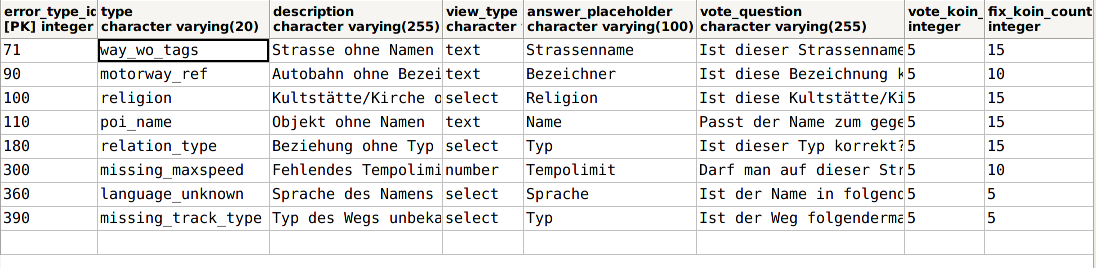
\includegraphics[scale=0.5]{images/backend/table-error-type}
	\caption{Die Tabelle \inlinecode{kort.error\_type}}
\end{figure}

\subsubsection{Erstellen eines neuen Fehlertyps}
\label{create-new-error-type}
Ein neuer Fehlertyp muss in der Tabelle \inlinecode{kort.error\_type} hinzugefügt werden.
Sobald Fehler als \inlinecode{type} den neuen Typ eingetragen haben, wird dieser auch angezeigt.
Jeder Fehlertyp hat ein zugehörige Marker-Icon welches beispielsweise auf der Karte angezeigt wird.
Die Bilddatei hat den gleichen Namen wie das Attribut \inlinecode{type} und befindet sich im Ordner \inlinecode{/resources/images/marker\_icons}.

\subsection{View-Typen}
\label{view-types}
All diese Typen werden dann wiederum einem spezifischen View-Typen zugeordnet.
Dieser bestimmt, wie das Formular zum Lösen des Fehlers in der Benutzeroberfläche aussieht.

In Tabelle \ref{kort-view-types-table} sind die bereits vorhandenen View-Typen beschrieben.

\begin{table}[H]
\centering
\begin{tabular}{|p{0.15\twocelltabwidth}|p{0.85\twocelltabwidth}|}
\hline
\textbf{Typ} & \textbf{Beschreibung} \\
\hline
\inlinecode{text} & Rendert ein Text-Eingabefeld \\
\hline
\inlinecode{number} & Rendert ein Zahl-Eingabefeld \\
\hline
\inlinecode{select} & Rendert eine Select-Box mit vorgefüllten Werten aus der Datenbank \\
\hline
\end{tabular}
\caption{kort: View-Typen}
\label{kort-view-types-table}
\end{table}

Wird als View-Typ \emph{select} gewählt, müssen in der Tabelle \inlinecode{kort.answer} noch die möglichen Antworten eingetragen werden.
Darin kann der eigentliche Wert des OpenStreetMap-Tags und eine passende Bezeichnung hinterlegt werden.
Als \inlinecode{type} muss der jeweilige Typen-Bezeichner gewählt werden.

\subsubsection{Erstellen eines neuen View-Typen}
Um einen neuen View-Typen zu definieren muss wie in Code-Ausschnitt \ref{kort-add_view_type} beschrieben die Unterscheidung in der Klasse \inlinecode{Kort.view.bugmap.fix.Form} um den neuen Typen ergänzt werden.

\lstset{language=JavaScript}
\begin{lstlisting}[float, caption=Hinzufügen eines View-Typen in der Klasse Kort.view.bugmap.fix.Form, label=kort-add_view_type]
createFixField: function(bug) {
	[...]
	
	if(bug.get('view_type') === '<Neuer View-Typ>') {
		fixField = Ext.create('<Neue View-Klasse>', fieldConfig);
	} else {
		...
	}
	
	[...]
}
\end{lstlisting}

\section{Hinzufügen von Auszeichnungen}
\label{kort-additional-badges}
Die bereits vorhandenen Auszeichnungen sind in Tabelle \ref{kort-badges} beschrieben. Um weitere Auszeichnungen hinzuzufügen, muss folgendermassen vorgegangen werden:

\begin{enumerate}
\item Es muss ein neuer \gls{Badge} in der Tabelle \inlinecode{kort.badge} erstellt werden
\item Zusätzlich muss eine Regel für das Gewinnen des \gls{Badge}s in der Methode \inlinecode{RewardHandler::updateBadges()}\footnote{\url{http://kort.herokuapp.com/docs/Kort-backend/classes/Webservice.RewardHandler.html\#method_updateBadges}} hinzugefügt werden.
\item Für das Frontend muss ein Bild erstellt werden, welches dem Namen (Tabellenattribut \inlinecode{kort.badge.name}) des \gls{Badge}s entspricht. Dieses Bild muss in folgendem Pfad gespeichert werden \inlinecode{/resources/images/badges/<badgename>.png}.
\end{enumerate}

Sind alle Punkte abgearbeitet ist der \gls{Badge} im Frontend ersichtlich und kann von den Benutzern gewonnen werden.

\section{Hinzufügen von OAuth Anbietern}
\label{kort-additional-oauth-provider}
Derzeit ist der Login über Googles \gls{OAuth}-Dienst möglich, um zukünftig weitere Login-Dienste anbieten zu können müssen einige Schritte beachtet werden.
Der Dienst muss folgende Anforderungen erfüllen:
\begin{itemize}
\item Unterstützung für OAuth 1.0 oder 2.0
\item Offline-Zugang, d.h. es müssen Aktionen ohne den Benutzer möglich sein
\item Ein längerfristig gültiges Token, welches als \emph{Refresh Token} bezeichnet wird
\item Der Dienst muss eine Registrierung der Applikation ermöglichen
\end{itemize}

Wenn ein Dienst diese Anforderung erfüllt, muss die Applikation registriert werden.
Die Angaben für Google sind dabei im Kapitel \ref{oauth} vermerkt.

Im Backend kann eine entsprechende Subklasse von \inlinecode{AbstractOAuthCallback}\footnote{\url{http://kort.herokuapp.com/docs/Kort-backend/classes/OAuth.AbstractOAuthCallback.html}} erstellt werden. 
Eine so erstellte OAuthCallback-Klasse nimmt dann einen Callback des entsprechenden Anbieters entgegen und authentifiziert den Benutzer.
Das zugehörige Callback-Script wird im Order \inlinecode{/server/oauth2callback} gespeichert.

Schlussendlich muss das Frontend noch angepasst werden.
Dazu gehört, dass der neue Dienst in der Konfiguration (siehe Kapitel \ref{frontend-config}) eingetragen werden muss.
Um einen neuen Login-Button anzuzeigen muss dieser auch noch auf dem Login-Panel (\inlinecode{/app/view/overlay/login/Panel.js}) hinzugefügt werden.
Die zugehörige Logik befindet sich im Login-Controller (\inlinecode{/app/controller/Login.js}).
\begin{figure}[H]
	\centering
	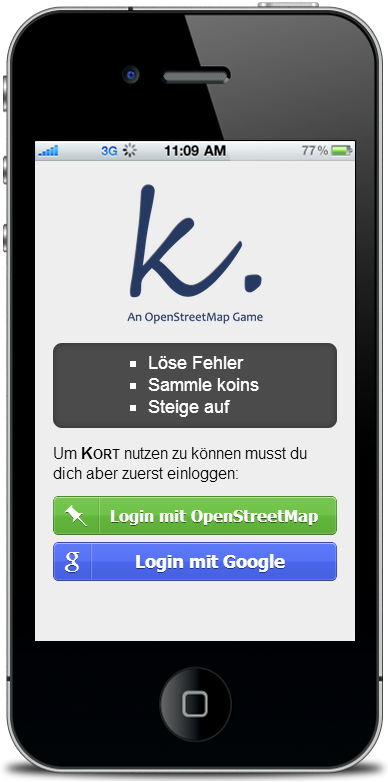
\includegraphics[scale=0.5]{images/screenshots/kort-screenshot-login}
	\caption{Login-Button des OAuth-Anbieters}
\end{figure}


\section{Reset der Applikation}
\label{kort-reset}
Um die Applikation zurückzusetzen kann die Stored Procedure \inlinecode{reset\_kort()} verwendet werden. 
Die Prozedur löscht alle laufenden Daten aus der Datenbank, so dass wieder der Ursprungszustand hergestellt ist:
\begin{itemize}
\item Die Punkte (\emph{\gls{koins}}) aller Benutzer werden auf 0 zurückgesetzt
\item Die \gls{Badge}s aller Benutzer werden entfernt
\item Alle Lösungsvorschläge von Benutzern werden entfernt
\item Alle Überprüfungen von Lösungsvorschlägen werden entfernt
\end{itemize}

Auf Aufruf der Prozedur sieht wiefolgt aus:
\begin{lstlisting}[float, caption=Aufruf von reset\_kort() um die Applikation zurückzusetzen, label=kort-reset-cmd]
select reset_kort();

 reset_kort 
------------
 t
(1 row)
\end{lstlisting}

Die Prozedur liefert \inlinecode{true} wenn alles geklappt hat, ansonsten \inlinecode{false}.

\section{Frontend Kofiguration}
\label{frontend-config}
Die Konfiguration des Frontends befindet sich in der Datei \inlinecode{/app/util/Config.js}.
Darin sind alle Parameter definiert, welche die Applikation für den Betrieb benötigt.

In der \textsc{Kort}-Dokumentaton sind alle Parameter detailliert beschrieben: \url{http://kort.herokuapp.com/docs/Kort/#!/api/Kort.util.Config}

% Neue Seite beginnen
\cleardoublepage

% Implementation
% Titel auch in Kopfzeile anzeigen
\markboth{Teil III. Implementation}{Teil III. Implementation}
\part{Implementation}
\section{Implementation}
\label{backend-implementation}
Das Backend besteht neben der Datenbank und den \gls{REST}-Schnittstellen vor allem aus PHP-Code.
Der meiste Code entfällt auf das Handling von Webservice-Anfragen und die Authentifizierung mit \gls{OAuth}.

\subsection{Gliederung}
\label{backend-gliederung}
Das Backend befindet sich im Verzeichnis \inlinecode{server/} im Repository.
Das Backend teilt sich auf verschiedene Unterordner auf (siehe Tabelle \ref{table-backend-gliederung}).

\begin{table}[H]
\centering
\begin{tabular}{|p{0.25\twocelltabwidth}|p{0.75\twocelltabwidth}|}
\hline 
\textbf{Order} & \textbf{Inhalt} \\
\hline 
\inlinecode{database/} & SQL und Shell-Skripts für die Erstellung der Datenbank \\
\hline 
\inlinecode{heroku/} & Shell-Skripte für das Deployment auf Heroku \\
\hline 
\inlinecode{oauth2callback/} & Callback-Handler der verschiedenen \gls{OAuth}-Dienste \\
\hline 
\inlinecode{php/} & PHP-Klassen für das Backend \\
\hline 
\inlinecode{redmine/} & Skripts und Anleitung für Redmine \\
\hline 
\inlinecode{ssh\_pub\_keys/} & Öffentliche SSH-Schlüssel für das Deployment \\
\hline 
\inlinecode{webservices/} & \gls{REST}-Ressourcen (Endpunkte der Schnittstellen) \\
\hline 
\end{tabular}
\caption{Gliederung des Backends}
\label{table-backend-gliederung}
\end{table}

Speziell zu erwähnen sind dabei die PHP-Klassen welche die Logik des Backends abbilden.
Sie sind über Namespaces aufgeteilt und liefern die Logik für alle anderen Teile des Backends.
Um dies zu ermöglichen gibt es die \inlinecode{ClassLoader}-Klasse\footnote{\url{http://kort.herokuapp.com/docs/Kort-backend/classes/Kort.ClassLoader.html}}.
Falls irgendwo eine PHP-Klasse gebraucht wird, muss nur diese Klasse geladen werden, diese wiederum kümmert sich darum, alle abhängigen Datei nachzuladen.

Für die Klassen gibt es eine separate Dokumentation (siehe Abschnitt \ref{backend-dokumentation}).

\subsection{Abhängigkeiten}
\label{backend-abhaengigkeiten}

\begin{table}[H]
\centering
\begin{tabular}{|p{0.35\threecelltabwidth}|p{0.15\threecelltabwidth}|p{0.50\threecelltabwidth}|}
\hline 
\textbf{Library} & \textbf{Version} & \textbf{Verwendung} \\
\hline 
Slim & 2.1.0 & Micro-Framework für die Implementation von \gls{REST}-Schnittstellen \\
\hline 
Google APIs Client Library & 0.6.0 & PHP-Library für Google \glspl{API} \\
\hline 
oauth-php & 175 & \gls{OAuth} Library für PHP \\
\hline 
Ant-Contrib & 1.0b3 & Erweiterte Tasks für Apache Ant \\
\hline 
\end{tabular}
\caption{Abhängigkeiten im Backend}
\label{table-backend-dependencies}
\end{table}



% Neue Seite beginnen
\cleardoublepage

% Projektmanagement
% Titel auch in Kopfzeile anzeigen
\markboth{Teil IV. Projektmanagement und -monitoring}{Teil VI. Projektmanagement und -monitoring}
\part{Projektmanagement und -monitoring}
% Projektmanagement
\chapter{Projektmanagement}
\label{projektmanagement}

Wir verwendeten die agile Projektmethodologie \emph{Scrum}\footnote{\url{http://www.scrum.org}} und arbeiteten dabei während 12 Wochen.
Die Dauer eines Sprints haben wir auf 2 Wochen festgelegt. Daraus ergeben sich insgesamt 6 Sprints.

\subsubsection{Aufwand pro Person}
Für diese Bachelorarbeit werden 12 ECTS-Punkte vergeben, wobei 1 ECTS-Punkt 30 Stunden Arbeitsaufwand bedeuten.
Dies ergibt 360 Stunden pro Person, was etwas mehr als 3 Arbeitstagen pro Woche entspricht.

\subsubsection{Anpassung der Sprintdauer}
Wir mussten während des Verlaufs des Projektes feststellen, dass die Sprintdauer von 2 Wochen etwas zu kurz ist und haben deshalb die letzten 3 Sprints (à 2 Wochen) durch 2 Sprints à 3 Wochen ersetzt. Insgesamt wurden deshalb im Projekt 5 Sprints durchgeführt. 

\subsubsection{Storypoints pro Sprint}
Als Ausgangslage haben wir 12 Storypoints pro Sprint angenommen, wobei 1 Storypoint ungefähr einem Arbeitstag entspricht. 
Dieser Wert hat sich gut bewährt und wir mussten ihn lediglich bei der Anpassungen der Sprintdauer auf 17 Punkte erhöhen.

% Sprints
\section{Sprints}

% Sprint 1
\input{body/projektmanagement_monitoring/sprint1.tex}

% Sprint 2
\input{body/projektmanagement_monitoring/sprint2.tex}

% Sprint 3
\input{body/projektmanagement_monitoring/sprint3.tex}

% Sprint 4
\input{body/projektmanagement_monitoring/sprint4.tex}

% Sprint 5
\input{body/projektmanagement_monitoring/sprint5.tex}


% Projektmonitoring
\chapter{Projektmonitoring}
\label{projektmonitoring}

% Meilensteine
\section{Meilensteine}
\label{meilensteine}

Um den Projektverlauf zu beurteilen, haben wir folgende Meilensteine erstellt:

\subsubsection{Meilenstein 1: Aufbereiten von Fehlerdaten}
\tick Geeignete Fehler finden \\
\tick Fehler in Datenbank speichern \\
\tick Fehler filtern \\
\tick Fehler zugänglich machen

\subsubsection{Meilenstein 2: Lesen von Fehlerdaten}

\tick Zugriff auf Datenbank aus App \\
\tick Persistieren der Daten in App

\subsubsection{Meilenstein 3: Kartenanzeige von Fehlern}

\tick Geeignete Kartendarstellung von Fehler finden \\
\tick Fehler auf der Karte anzeigen \\
\tick Location-based Karte

\subsubsection{Meilenstein 4: OAuth}

\tick Login möglich über OAuth \\
\tick User wird in App persistiert \\
\tick Logout möglich \\
\cross Login mit OSM-OAuth

\subsubsection{Meilenstein 5: Schreiben von Fehlerbehebungen}

\tick Input von User speichern in DB \\
\tick Unterscheidung von Fehlertypen

\subsubsection{Meilenstein 6: Verifizieren von Änderungen}

\tick UI zum verifizieren von Fehlerbehebungen \\
\cross Implementation eines Thresholds für Verfikationen

\subsubsection{Meilenstein 7: Daten zu OSM schicken}

\cross Verifikationsdaten einheitlich via API an OSM senden \\
\cross Prüfung ob eine Änderung zulässig ist

\subsubsection{Meilenstein 8: Gamification-Konzepte (Highscore, Leaderboard, Badges, Achievements)}

\cross Erarbeitung eines Gamifications-Konzepts für OSM \\
\tick Geeignete Elemente in App umsetzen (\tick Highscore, \tick Badges)

% Risikomanagement
\section{Risikomanagement}
\label{risikomanagement}

Für das Projekt wurden folgende Risiken identifiziert:
\subsection{Technische Risiken}

\subsubsection{OpenStreetMap-Daten können nicht in einer Sencha Touch-Applikation angezeigt werden}
\begin{table}[H]
\centering
\begin{tabular}{|p{0.25\twocelltabwidth}|p{0.75\twocelltabwidth}|}
\hline 
\small{\textbf{Auswirkung}} & Es müsste ein alternatives mobiles Framework gefunden werden, welches mit \brand{OpenStreetMap}-Daten umgehen kann. \\
\hline 
\small{\textbf{Wahrscheinlichkeit}} & tief \\
\hline 
\small{\textbf{Massnahme zur Verhinderung}} & Zu Beginn des Projektes muss eine Sencha Touch Prototyp-Applikation implementiert werden, welche \brand{OpenStreetMap}-Daten auf der Karte darstellt. \\
\hline
\end{tabular}
\end{table}

\subsubsection{Keine geeignete Fehlerdatenquelle vorhanden}
\begin{table}[H]
\centering
\begin{tabular}{|p{0.25\twocelltabwidth}|p{0.75\twocelltabwidth}|}
\hline 
\small{\textbf{Auswirkung}} & Es müsste eine Möglichkeit gefunden werden, vorhandene Fehlerdaten so abzuändern, dass sie für den Einsatz in der App verwendet werden können. \\
\hline 
\small{\textbf{Wahrscheinlichkeit}} & mittel \\
\hline 
\small{\textbf{Massnahme zur Verhinderung}} & Es muss eine Evaluation von bestehenden Fehlerdatenquellen durchgeführt werden. \\
\hline
\end{tabular}
\end{table}

\subsubsection{Schwierigkeiten mit OAuth}
\begin{table}[H]
\centering
\begin{tabular}{|p{0.25\twocelltabwidth}|p{0.75\twocelltabwidth}|}
\hline 
\small{\textbf{Auswirkung}} & OAuth ist als Protokoll bekannt, welches Schwierigkeiten bereiten kann.
Falls sich die Anforderungen nicht umsetzen lassen, muss eine alternative Lösung gefunden werden für den Login. \\
\hline 
\small{\textbf{Wahrscheinlichkeit}} & mittel \\
\hline 
\small{\textbf{Massnahme zur Verhinderung}} & Wir müssen genügend Zeit für OAuth einplanen. \\
\hline
\end{tabular}
\end{table}

\subsection{Weitere Risiken}

\subsubsection{OpenStreetMap erlaubt keinen allgemeinen Benutzer zum Zurückschreiben der Fehlerbehebungen}
\begin{table}[H]
\centering
\begin{tabular}{|p{0.25\twocelltabwidth}|p{0.75\twocelltabwidth}|}
\hline 
\small{\textbf{Auswirkung}} & Es müsste eine Möglichkeit gefunden werden, die Fehlerbehebungen trotzdem in \brand{OpenStreetMap} einpflegen zu können \\
\hline 
\small{\textbf{Wahrscheinlichkeit}} & mittel \\
\hline 
\small{\textbf{Massnahme zur Verhinderung}} & \brand{OpenStreetMap}-Community muss von der Idee hinter \kort{} überzeugt werden. \\
\hline
\end{tabular}
\end{table}

\subsubsection{Zu wenig Erfahrung mit Game-Design}
\begin{table}[H]
\centering
\begin{tabular}{|p{0.25\twocelltabwidth}|p{0.75\twocelltabwidth}|}
\hline 
\small{\textbf{Auswirkung}} & Die App hat keinen Game-Charakter oder wird vom Benutzer nicht als solches erkannt. \\
\hline 
\small{\textbf{Wahrscheinlichkeit}} & gross \\
\hline 
\small{\textbf{Massnahme zur Verhinderung}} & Unser Industriepartner hat viel Erfahrung mit der Entwicklung von Games und kann uns mit Ratschlägen unterstützen.
Daneben haben wir versucht, Designer zu involvieren welche uns unterstützen können. \\
\hline
\end{tabular}
\end{table}

\section{Projektverlauf}
Das Projekt bestand aus 5 Sprints, wobei wir ursprünglich 6 geplant haben.
Gegen Ende des Projekts mussten wir uns eingestehen, dass der Overhead für zweiwöchige Sprints zu gross ist, deshalb haben wir die letzten beiden Sprints auf 3 Wochen erweitert.

Dank \brand{Redmine}, unsere Projektmanagement-Tool, hatten wir eine gute Übersicht über das Projekt.
Jeweils am Ende eines Sprints haben wir besprochen wie wir weiterfahren sollen und haben entsprechend den nächsten Sprint geplant.
Durch diese Iterationen war es uns möglich, schnell ein System zu erstellen, welches den aktuellen Bedürfnissen entspricht.

Im Laufe des Projeks hat es sich ergeben, dass sich Herr Hunziker eher um das Frontend und Herr Oderbolz eher um das Backend gekümmert hat.
Die Grenzen sind dabei fliessend und sind grösstenteils durch die persönlichen Interessen entstanden.
Da wir das Studium berufsbegleitend absolvieren und uns deshalb nicht jeden Tag getroffen haben, hatte dies den Vorteil, dass wir so relativ gut unabhängig voneinander arbeiten konnten.

Etwa in der Hälfe des Projekts wollte unser Betreuer Prof. Stefan Keller wissen, welche Funktionalitäten wir bis zum Ende abschliessen können und welche nicht.
Die agile Vorgehensweise erlaubt es grundsätzlich nicht solche Aussagen zu treffen, da sich der Scope noch ändern kann.
Jedoch ist es natürlich verständlich, dass man eine Übersicht will wie das Projekt vorangeschritten ist.
Deshalb haben wir dann begonnen eine Meilenstein-Liste zu führen, welche die wichtigsten Funktionalitäten aufzeigt.
So konnten wir zum einen jeweils zeigen, was schon erledigt und was noch zu tun ist und zum anderen jeweils beim Sprint Planning direkt Meilensteine einplanen.

Abschliessend ist zu sagen, dass das Projekt gut verlaufen ist, und wir grundsätzlich alle unsere Ziele erreichen konnten (siehe Abschnitt \ref{fazit}).
Daneben gab es auch Raum um kreative Ideen auszuprobieren.

\section{Arbeitsaufwand}
Wie im Kapitel \ref{projektmanagement} beschrieben, war der vom Modul vorgegebene Aufwand pro Person auf \emph{320 Stunden} festgelegt. Leider haben wir beide diese Vorgabe leicht überschritten (siehe Tabelle \ref{projektmanagement-arbeitsaufwand}).
\todo[inline]{Beschreibung Arbeitsaufwand}

\begin{table}[H]
\centering
\begin{tabular}{|l|l|}
\hline 
\textbf{Person} & \textbf{Aufwand} \\ 
\hline 
Jürg Hunziker & 339h \\
\hline 
Stefan Oderbolz & 352h \\  
\hline 
\end{tabular}
\caption{Arbeitsaufwand pro Person}
\label{projektmanagement-arbeitsaufwand}
\end{table} 

\section{Fazit}
\label{fazit}
Bereits die Liste der Meilensteine (siehe Abschnitt \ref{meilensteine}) vermittelt ein ambitioniertes Ziel, welches zu erreichen war.
Leider konnten wir nicht alle Punkte abschliessen.
Schlussendlich haben wir uns auf die Grundfunktionalität der \gls{WebApp} konzentriert.
So mussten wir leider auf das Zurückschreiben der korrigierten Daten zu \brand{OpenStreetMap} verzichten.

Die entwickelte \gls{WebApp} erfüllt alle Erwartungen an eine moderne Applikation.
Ein Benutzer kann mit der App die gewünschten Aufgaben (Fehler korrigieren und validieren) durchführen und wird durch einige Gamification-Konzepte animiert die App weiter zu verwenden.

In der doch kurzen Zeit ist es uns aber nicht gelungen ein vollwertiges Spiel zu entwickeln.
Dazu müsste noch mehr Wert auf Details gelegt werden, so dass eine abgerundetes Spielerlebnis entsteht.

Dank der agilen Vorgehensweise konnten wir schnell auf Änderungen reagieren, welche sich bei einem solchen Projekt zwangläufig ergeben.
Wir waren uns zu beginn noch nicht bewusst, welche Funktionalitäten wichtig sind und welche weniger.
Der ursprüngliche Plan so schnell wie möglich einen Roundtrip durch alle Systeme zu erlangen.
Als wir gemerkt haben, dass wir es mit vielen verschiedenen Schnittstellen zu tun haben, sind wir von diesem Plan wieder abgekommen und haben uns dazu entschlossen, zuerst unsere App zu stabilisieren und dann eine Schnittstelle nach der anderen anzuschauen.

Mit Hilfe der \gls{ci} hatten wir stets ein lauffähiges System welchen automatisiert gebaut und ausgerollt wurde.

% -----------------------------------------
% FOOT
% -----------------------------------------
% Neue Seite beginnen
\cleardoublepage

% Anhänge
% Titel auch in Kopfzeile anzeigen
\markboth{Teil V. Anhänge}{Teil V. Anhänge}
\part{Anhänge}

% Inhalt der CD
\chapter*{Inhalt der CD}
% Titel auch in Kopfzeile anzeigen
\markboth{Inhalt der CD}{Inhalt der CD}
% Kapitel in Inhaltsverzeichnis einfügen
\addcontentsline{toc}{chapter}{Inhalt der CD}

\begin{table}[H]
\centering
\begin{tabular}{|p{0.35\twocelltabwidth}|p{0.65\twocelltabwidth}|}
\hline 
\textbf{Pfad} & \textbf{Beschreibung} \\ 
\hline 
\inlinecode{.sencha/} & Konfiguration für Sencha Cmd \\ 
\hline 
\inlinecode{\_DESIGN/} & Grafik-Rohdaten \\ 
\hline 
\inlinecode{\_DOCUMENTATION/} & Dokumentation der Arbeit \\ 
\hline 
\inlinecode{\_DOCUMENTATION/ba-kort-
\newline jhunzike\_soderbol.pdf} & Dokumentation der Arbeit im PDF-Format \\ 
\hline 
\inlinecode{app/} & \textsc{Kort} Frontend \\ 
\hline 
\inlinecode{build/Kort/production/} & \textsc{Kort} Production Build (komprimierte JavaScript Sourcefiles) \\ 
\hline 
\inlinecode{docs/} & Generierte Code-Dokumentationen (\textsc{Kort} Frontend, \textsc{Kort} Backend, Ext.ux.LeafletMap) \\ 
\hline 
\inlinecode{i18n/} & Internationalisierungs-Plugin für Sencha Touch \\ 
\hline 
\inlinecode{jsduck/} & Konfiguration zur Gererierung der JSDuck Code-Dokumentation \\ 
\hline 
\inlinecode{lib/} & Verwendete Library-Pakete \\ 
\hline 
\inlinecode{resources/} & Ressourcen, welche von \textsc{Kort} verwendet werden (CSS, Bilder, Sprach-Property-Files) \\ 
\hline 
\inlinecode{server/} & \textsc{Kort} Backend \\ 
\hline 
\inlinecode{test/} & Tests der Use Cases und Libraries \\ 
\hline 
\inlinecode{touch/} & Sencha Touch 2 Library \\ 
\hline 
\inlinecode{ux/} & Sencha Touch Erweiterungs-Komponenten \\ 
\hline 
\inlinecode{app.js} & Einstiegspunkt des \textsc{Kort} Frontends \\ 
\hline 
\inlinecode{app.json} & Sencha Cmd Konfiguration von \textsc{Kort} \\ 
\hline 
\end{tabular}
\end{table}

% Glossar
\printglossary[style=altlist,title=Glossar,toctitle=Glossar]

% Literaturverzeichnis
\bibliographystyle{plainurl}
\bibliography{foot/literatur}

% Abbildungsverzeichnis
\listoffigures

% Tabellenverzeichnis
\listoftables

\end{document}